% !TEX program = xelatex
\documentclass[12pt,a4paper]{ctexart}
\usepackage[left=2.5cm,right=2.5cm,top=2.6cm,bottom=2.6cm]{geometry}
\usepackage{graphicx,booktabs,float,caption,hyperref,xcolor,listings,enumitem,setspace,amsmath,array}
\captionsetup{font=small,labelfont=bf,labelsep=space}
\setstretch{1.3}
\hypersetup{colorlinks=true,linkcolor=blue!50!black,urlcolor=blue!50!black}
\ctexset{
section={
name={第,章},
number=\chinese{section},
format=\centering\heiti\zihao{-2},
beforeskip=1.2ex,
afterskip=3.5ex
},
subsection={
format=\heiti\zihao{4},
beforeskip=1.0ex,
afterskip=0.8ex
},
subsubsection={
format=\heiti\zihao{-4},
beforeskip=0.8ex,
afterskip=0.6ex
}
}
\renewcommand{\contentsname}{目\quad 录}
\definecolor{codebg}{RGB}{248,250,252}
\definecolor{codekw}{RGB}{34,87,122}
\definecolor{codestr}{RGB}{174,92,48}
\definecolor{codecom}{RGB}{95,117,135}
\definecolor{codenum}{RGB}{120,120,120}
\lstdefinestyle{pythonstyle}{language=Python,backgroundcolor=\color{codebg},basicstyle=\ttfamily\small,keywordstyle=\color{codekw}\bfseries,stringstyle=\color{codestr},commentstyle=\color{codecom}\itshape,numbers=left,numberstyle=\scriptsize\color{codenum},frame=single,rulecolor=\color{black!35},breaklines=true,showstringspaces=false,tabsize=4,xleftmargin=1em,xrightmargin=0.4em,lineskip=-0.5pt}
\begin{document}
\sloppy

\begin{titlepage}
    \centering
    \vspace*{1cm}
    {\zihao{1}\heiti 变构飞行器领域知识图谱构建与可视化系统设计与实现 \par}
    \vspace{2cm}
    
\includegraphics[width=0.3\textwidth]{figures/Tjulogo.png} \par
    \vspace{3cm}
    {\zihao{3}\heiti
    \begin{tabular}{l}
        \makebox[4em][s]{学\hfill 院}：\underline{\makebox[180pt][c]{软件学院}} \\ \addlinespace[10pt]
        \makebox[4em][s]{成员 1}：\underline{\makebox[180pt][c]{于露雪\quad 3023244303}} \\ \addlinespace[10pt]
        \makebox[4em][s]{成员 2}：\underline{\makebox[180pt][c]{杨博文\quad 3023244317}} \\ \addlinespace[10pt]
        \makebox[4em][s]{班\hfill 级}：\underline{\makebox[180pt][c]{4班}} \\ \addlinespace[10pt]
        \makebox[4em][s]{年\hfill 级}：\underline{\makebox[180pt][c]{2023级}}
    \end{tabular} \par}
    \vfill
    {\zihao{4} \today \par}
\end{titlepage}

\newpage
\tableofcontents
\newpage

\newpage
\section{绪论}
\subsection{项目背景、发展现状及意义和目标的理解}
变构飞行器能够根据任务需求主动调整外形，是航空航天领域的重要研究方向。本项目旨在利用知识图谱技术对该领域的零散知识进行结构化组织，其核心逻辑可归纳为以下两个方面：

\begin{itemize}[leftmargin=2em, label=\textbullet]
    \item \textbf{行业背景与核心痛点：} 变构飞行器研究涉及气动、结构与控制等多个层面的深度耦合，其多学科交叉特征使得知识获取门槛较高。当前的发展现状表明，核心知识高度分散在海量文献中，存在严重的语义表达不一致和关联关系隐含等痛点，导致研究者在查找和复用知识时需要投入巨大的归纳成本。构建领域知识图谱能够将碎片化的“文献资料”转化为结构化的“知识网络”，从根本上解决知识载体分散与语义检索困难的问题。

    \item \textbf{建设意义与总体目标：} 本项目的研究意义在于通过“规则引擎 + 语义模型”的混合手段，提升专业领域知识获取的可解释性与工程可维护性。项目建设的总体目标是形成一套完整的技术管线：首先构建面向变构飞行器领域的术语与本体体系；其次实现高召回、高精度的实体关系稳定抽取；最后开发可交互的 Web 展示系统，并利用人工金标准对系统性能进行量化验证。通过这一闭环流程，希望实现一套兼顾规范性与工程落地性的领域知识组织原型。
\end{itemize}

\subsection{项目实施技术路线及方案}
本项目总体采用“文献输入—文本预处理—术语构建—知识抽取—图谱导出—系统展示—算法评估”的技术路线。系统以 Python 为核心开发语言，后端基于 FastAPI，前端基于 ECharts，文本处理与统计建模结合 PyMuPDF、pdfminer.six、jieba、pandas 等工具库，并在术语定稿阶段引入 OpenAI 兼容大模型接口。

与单一深度学习方案不同，本项目采用了双模混合智能（Hybrid）架构，即“统计方法 + 规则系统 + LLM 抽取与精筛”。在工程实现上，系统支持检测人工金标词典：当存在人工词典时，维持高标准、高可解释性的规则引擎；否则自动切换为全自动大语言模型模式，以此保证系统的学术可复现性与工程泛化性。此外，大语言模型不仅用于术语归一化和类型定稿，还被深度整合到上下文感知的关系抽取中，并辅以多线程并行调度（ThreadPoolExecutor）以突破调用瓶颈，这既避免了纯规则方法产生的图谱稀疏问题，又显著提升了大规模数据处理的并发效率。

为便于说明系统从原始文献到最终图谱展示的整体演化过程，图~\ref{fig:route} 给出了项目实施技术路线，重点展示了各阶段输入输出之间的衔接关系。读者可以据此把握本项目从数据获取、知识抽取到系统实现的总体流程。

\begin{figure}[H]\centering
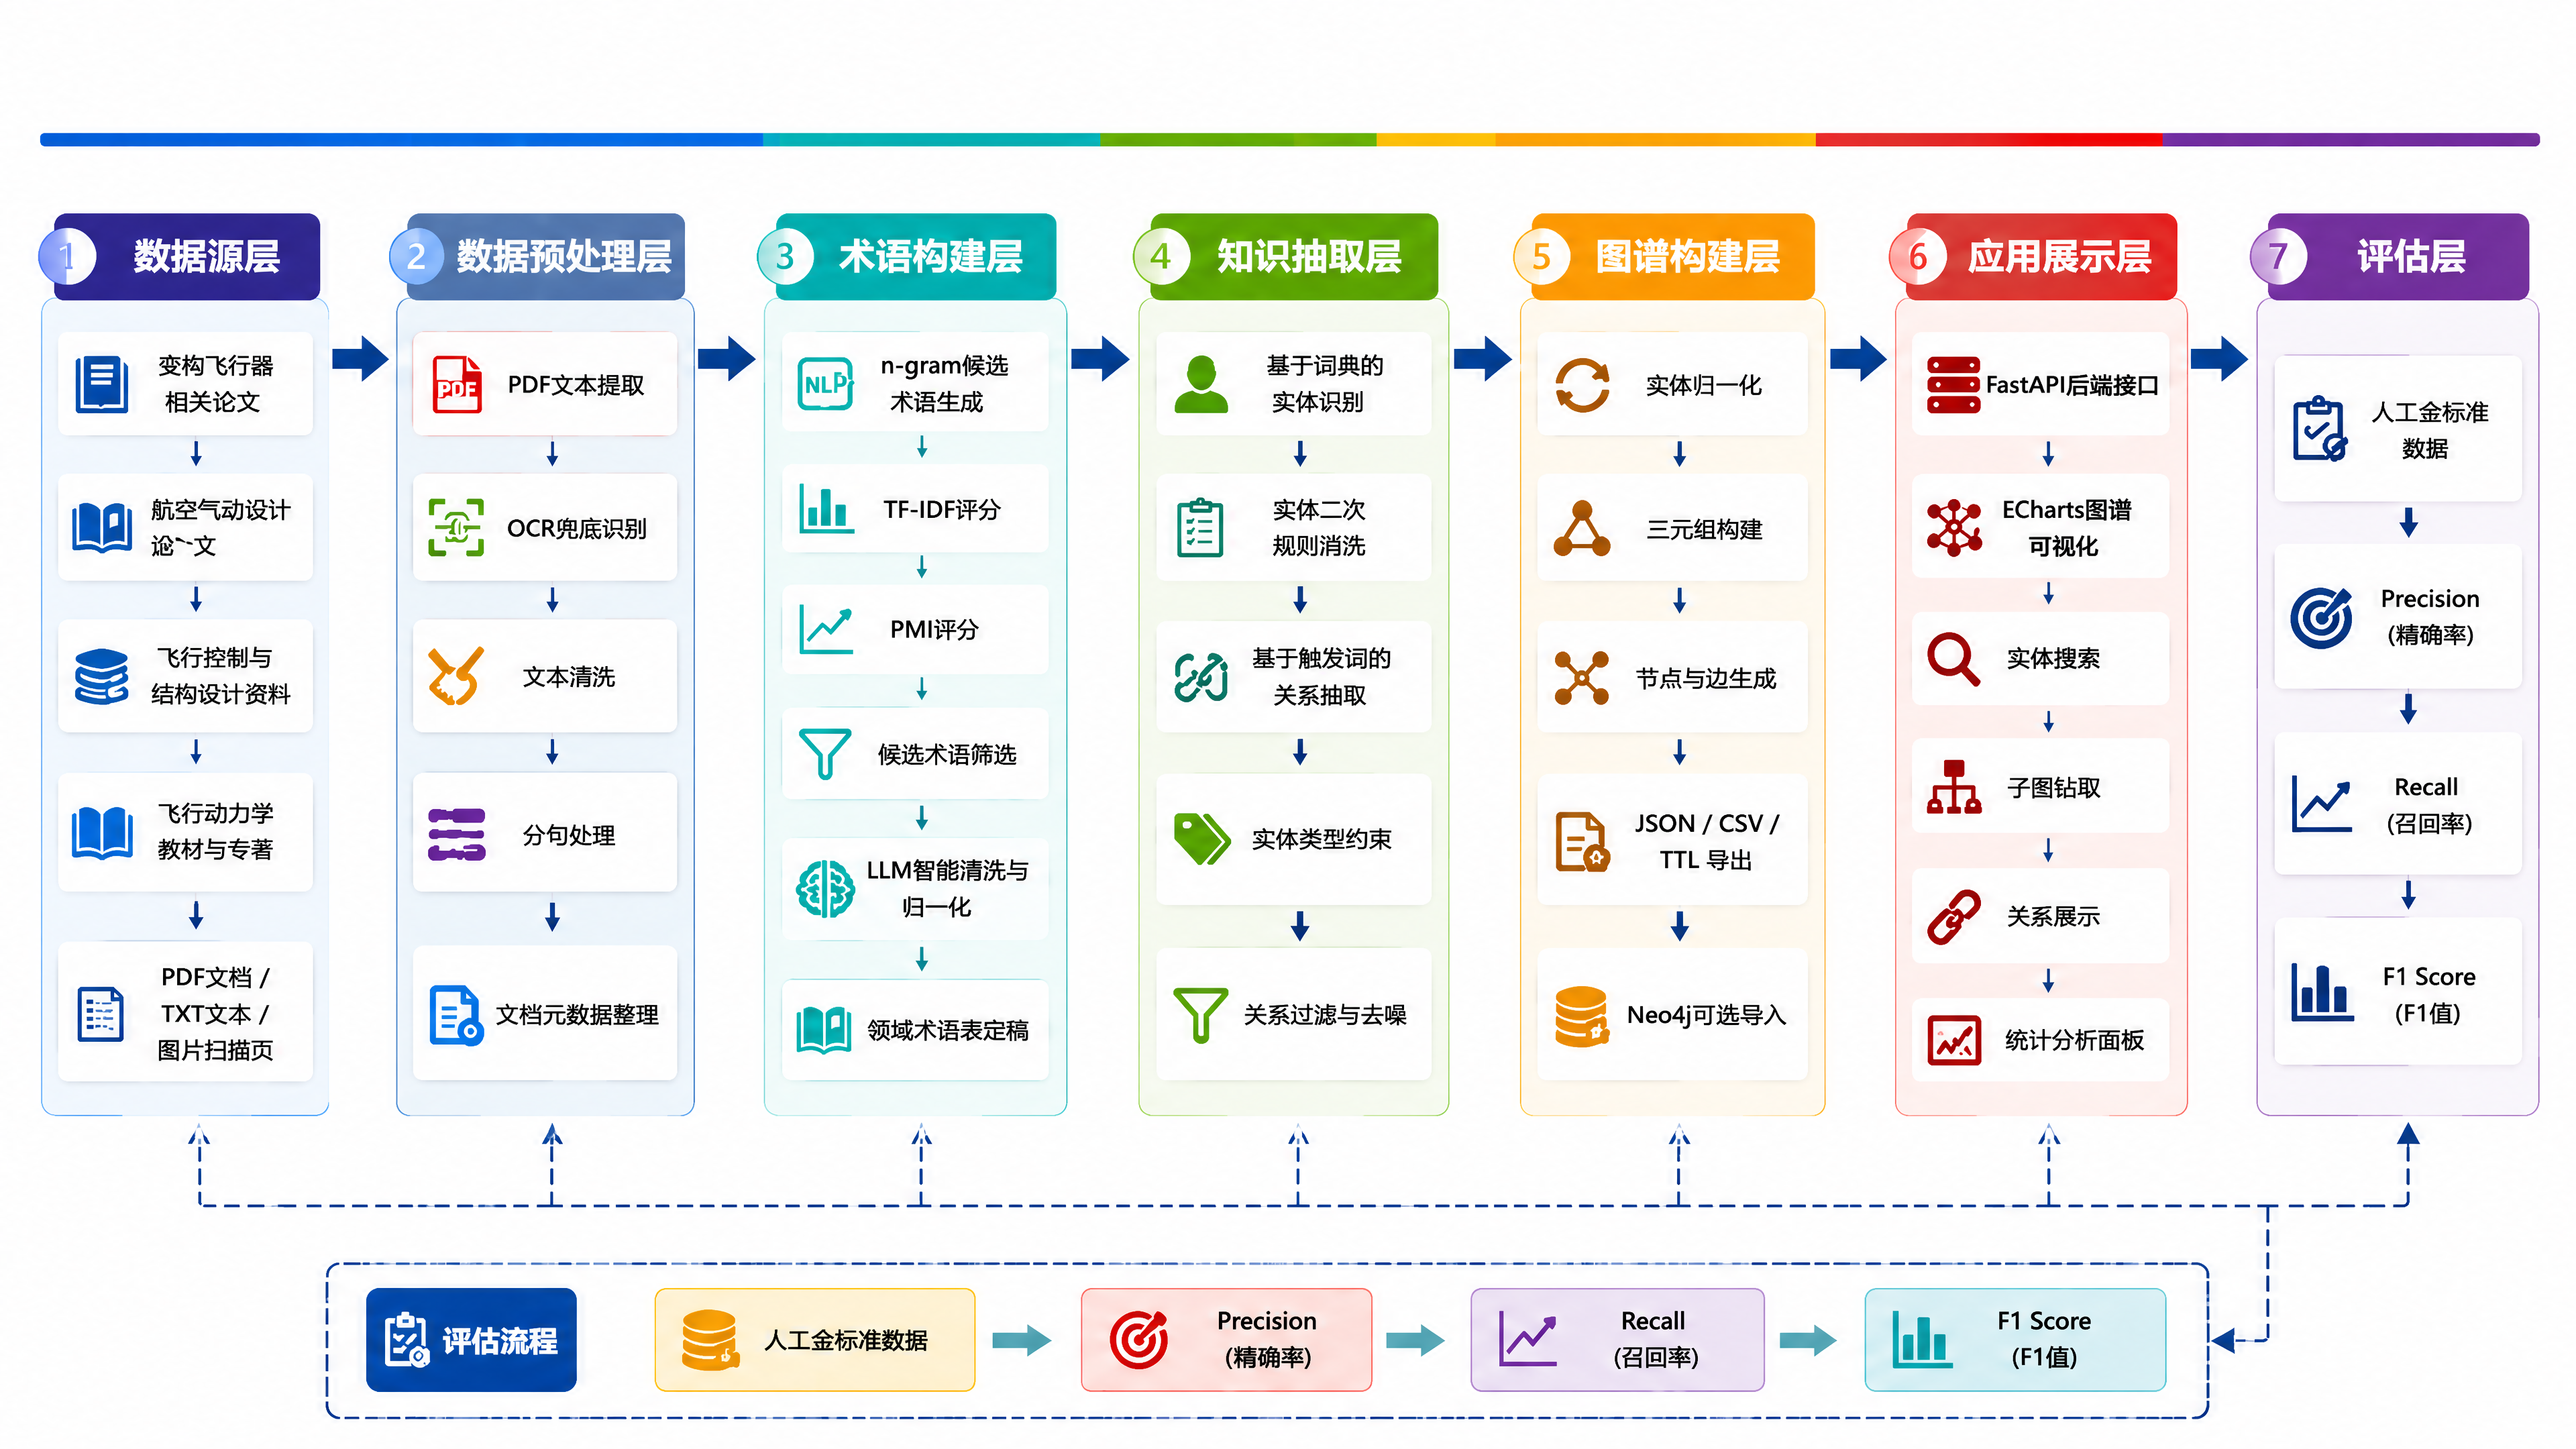
\includegraphics[width=0.90\textwidth]{figures/项目实施技术路线图.png}
\caption{项目实施技术路线图}
\label{fig:route}
\end{figure}

在总体流程明确之后，还需要进一步说明系统内部各模块的组织方式。图~\ref{fig:arch} 展示了系统总体架构，从数据层、处理层、抽取层到图谱层、服务层和展示层逐层展开，体现了本项目模块化、分层化的工程组织思路。

\begin{figure}[H]\centering
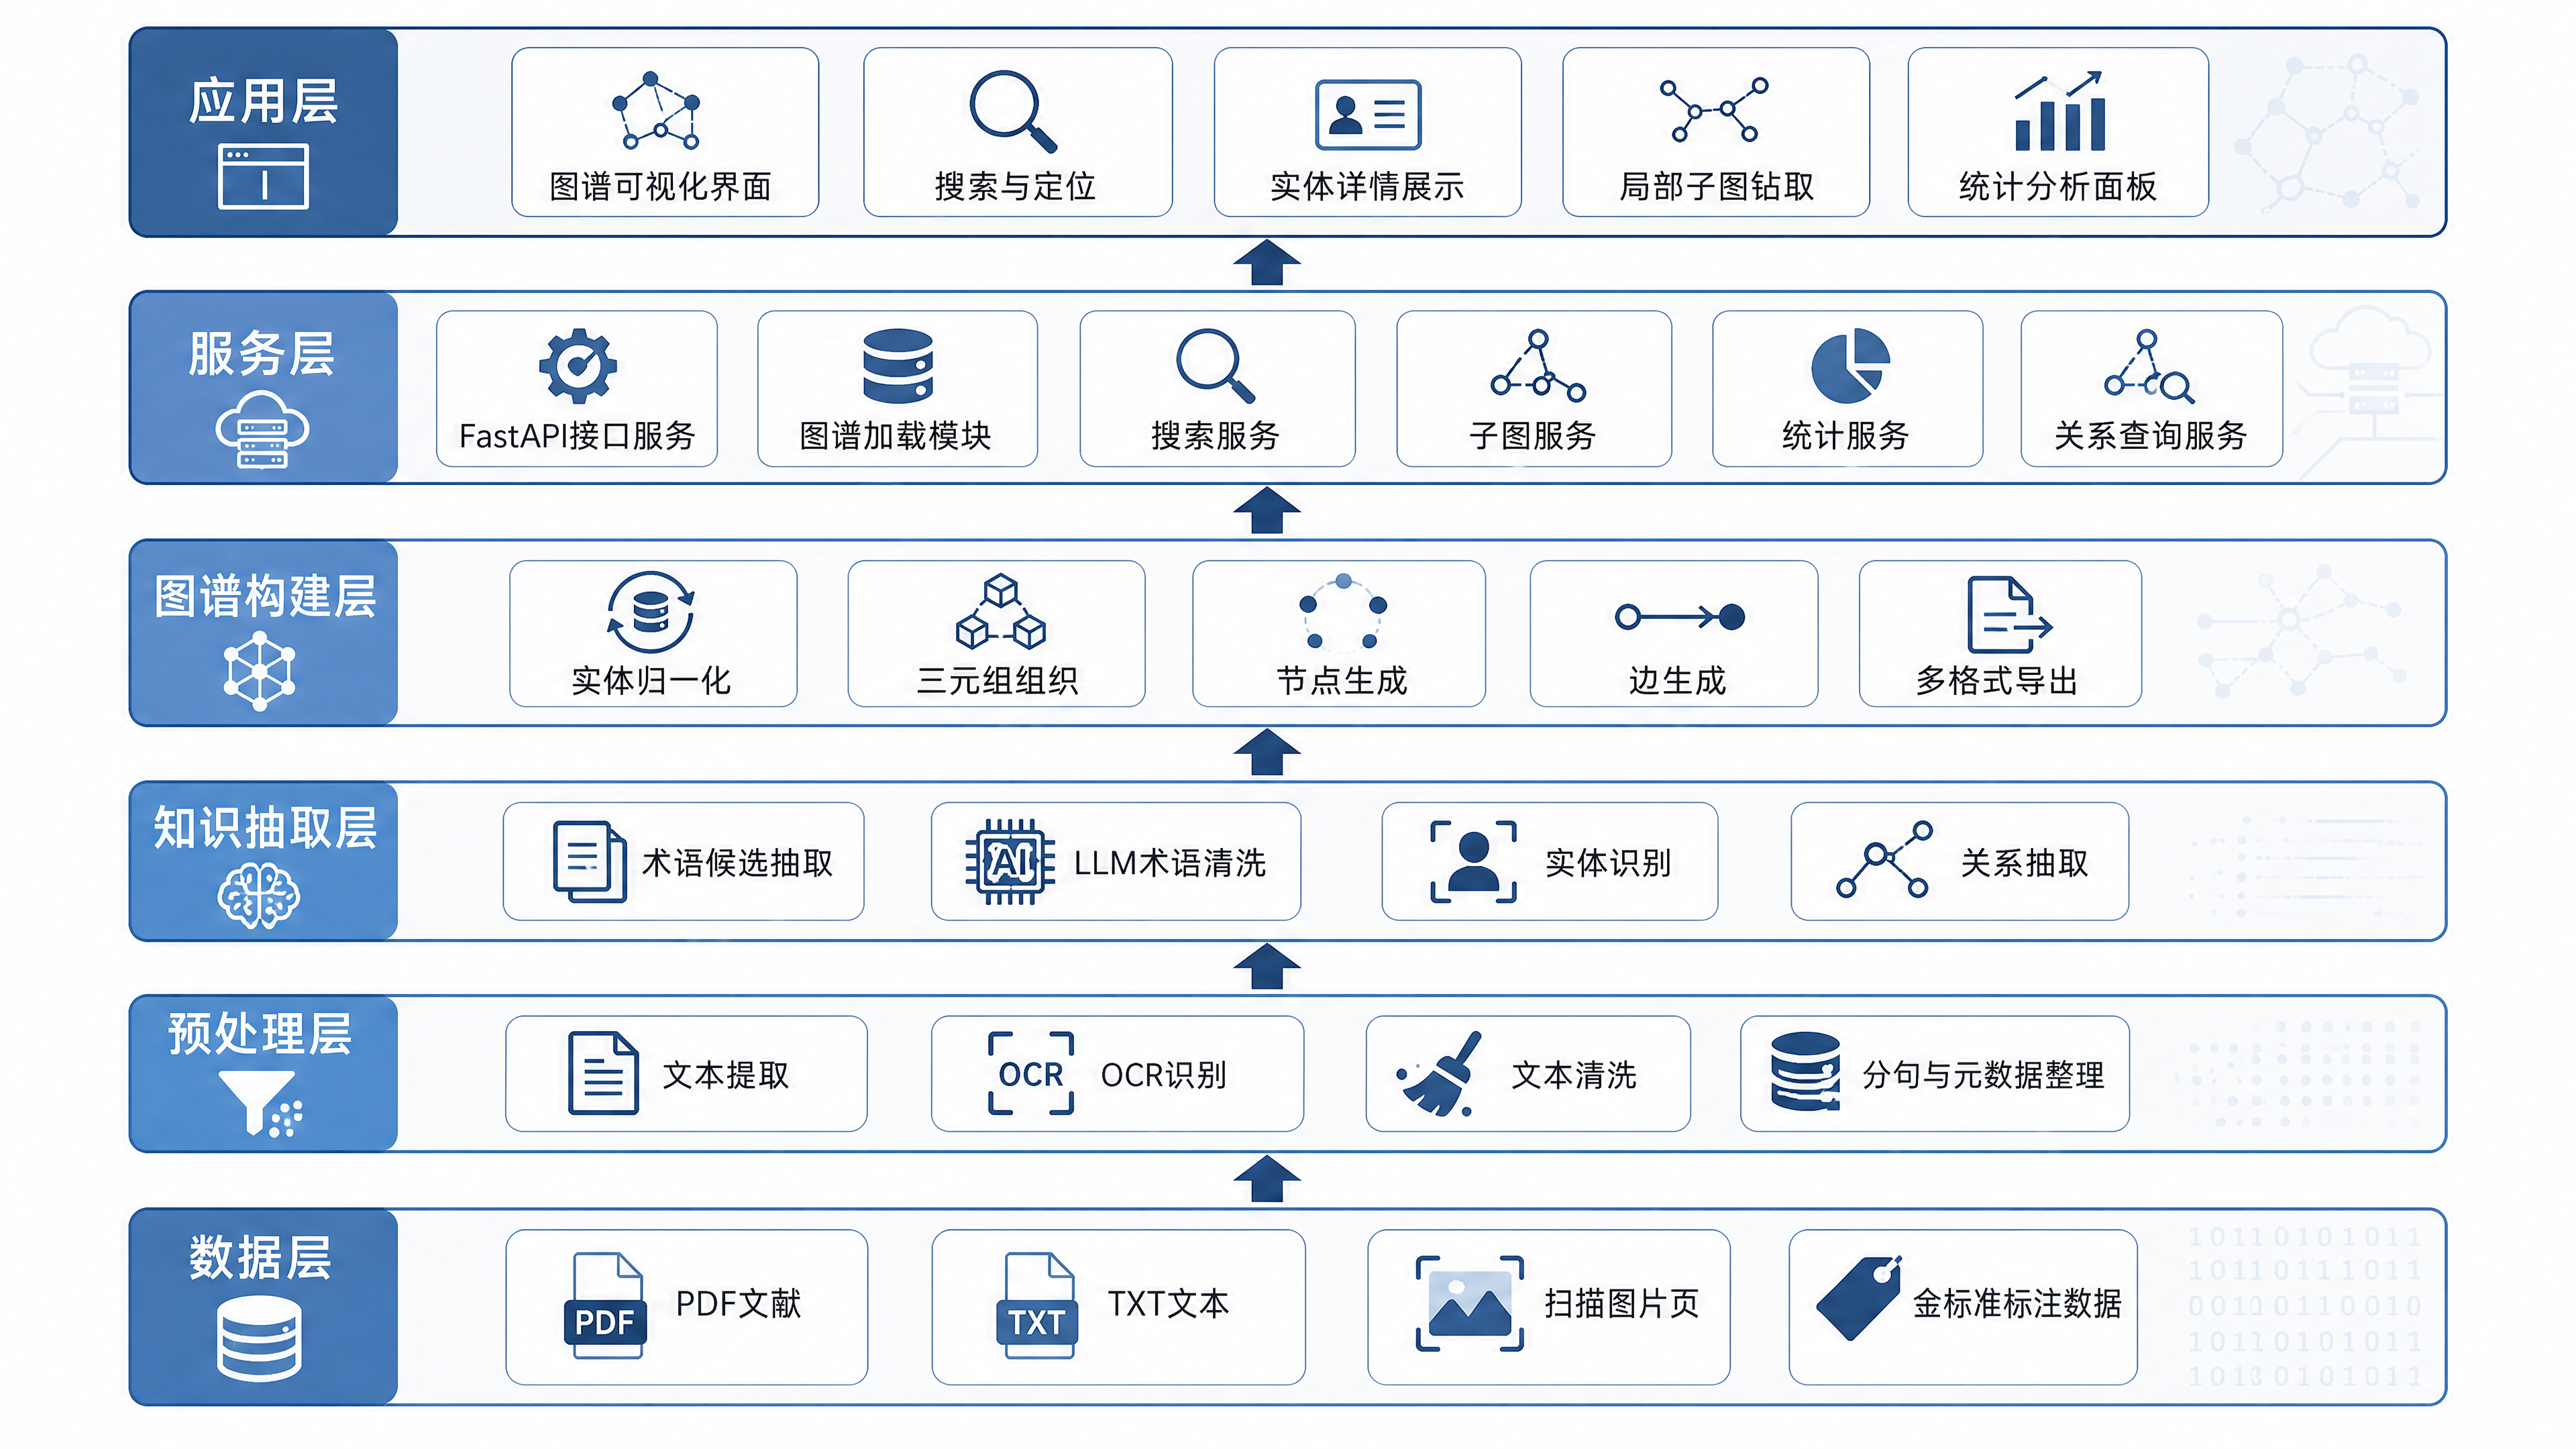
\includegraphics[width=0.86\textwidth]{figures/系统总体架构图.png}
\caption{系统总体架构图}
\label{fig:arch}
\end{figure}


\newpage
\section{数据源与信息获取}
\subsection{领域数据源梳理}
本项目的知识来源以变构飞行器领域中文文献为主，涵盖航空航天专著、结构设计资料、飞行控制文献、气动分析文献和综述性材料。数据形态以 PDF 为主，同时存在少量扫描页、编码异常页及纯文本中间语料。项目通过 \texttt{documents.csv} 管理文档元数据，通过 \texttt{data/text\_ascii/} 与 \texttt{data/processed/sentences.jsonl} 统一管理预处理结果，从而保证后续各阶段输入的一致性和可复用性。

从来源功能上看，不同类型文献在知识图谱构建中的作用并不相同。专著适合提供较稳定的概念定义、分类体系和组成结构信息；研究论文更容易提供新方法、新参数关系和实验结论；综述文献则适合抽取领域术语、研究热点和跨文献的概念对应关系。因此，在进行数据源梳理时，项目并未将所有文献等价处理，而是从知识贡献角度理解其价值。换言之，数据源不仅是算法输入，更直接影响后续实体类型设计、关系模式覆盖范围以及图谱最终的知识密度。

从知识结构看，专著更适合提供系统性的概念层次与结构组成知识，期刊论文更适合提供参数影响、控制方法和性能分析关系，综述文献则有助于归纳领域术语体系与主要研究方向。因此，数据源梳理不仅是语料准备过程，也是后续本体设计和关系模式抽取的重要基础。

此外，原始文献在格式层面差异较大。部分 PDF 具有清晰的文本层，适合直接抽取；部分资料为扫描型页面，需要 OCR 识别；还有一些文献虽然可抽出文本，但存在严重断行、乱码、页眉页脚干扰和图表内容混入等问题。这意味着领域知识获取不能简单理解为“读取 PDF 文本”，而应被视为一项涵盖文档治理、质量控制与中间结果标准化的前处理工程。正因为本项目在数据源阶段对这些问题进行了专门设计，后续术语抽取和实体关系抽取才能获得相对稳定的输入基础。

\subsection{关键信息获取方法}
\subsubsection{面向 PDF 文献的文本提取方法}
针对中文学术 PDF 常见的编码异常、文本层混乱和扫描页问题，项目在 \texttt{preprocess/extract.py} 中设计了三级容错策略：优先使用 PyMuPDF 提取文本层；若文本质量不佳，则回退至 \texttt{pdfminer.six} 进行细粒度解析；若仍无法获得有效文本，则使用 OCR 视觉模型进行兜底识别。其核心思想是优先采用成本较低、保真度较高的抽取方式，仅在必要时升级到更强但更慢的方案。

设文档页为 \(d\)，文本质量阈值为 \(\tau\)，则可将策略抽象表示为
\[
T^*(d)=\begin{cases}T_1(d), & q_1\ge\tau \\ T_2(d), & q_1<\tau,\ q_2\ge\tau \\ T_3(d), & q_1<\tau,\ q_2<\tau\end{cases}
\]
其中 \(T_1,T_2,T_3\) 分别对应 PyMuPDF、pdfminer 和 OCR 方法，\(q_1,q_2\) 为文本质量评分。该分层处理方式兼顾了效率与鲁棒性。

为了更直观地展示文本获取和数据清洗的先后关系，图~\ref{fig:preprocess} 总结了从原始 PDF 输入到干净句子语料输出的关键处理环节。该图有助于说明本项目并不是单步抽取，而是通过多级容错和多步预处理逐渐提升文本可用性。

\begin{figure}[H]\centering
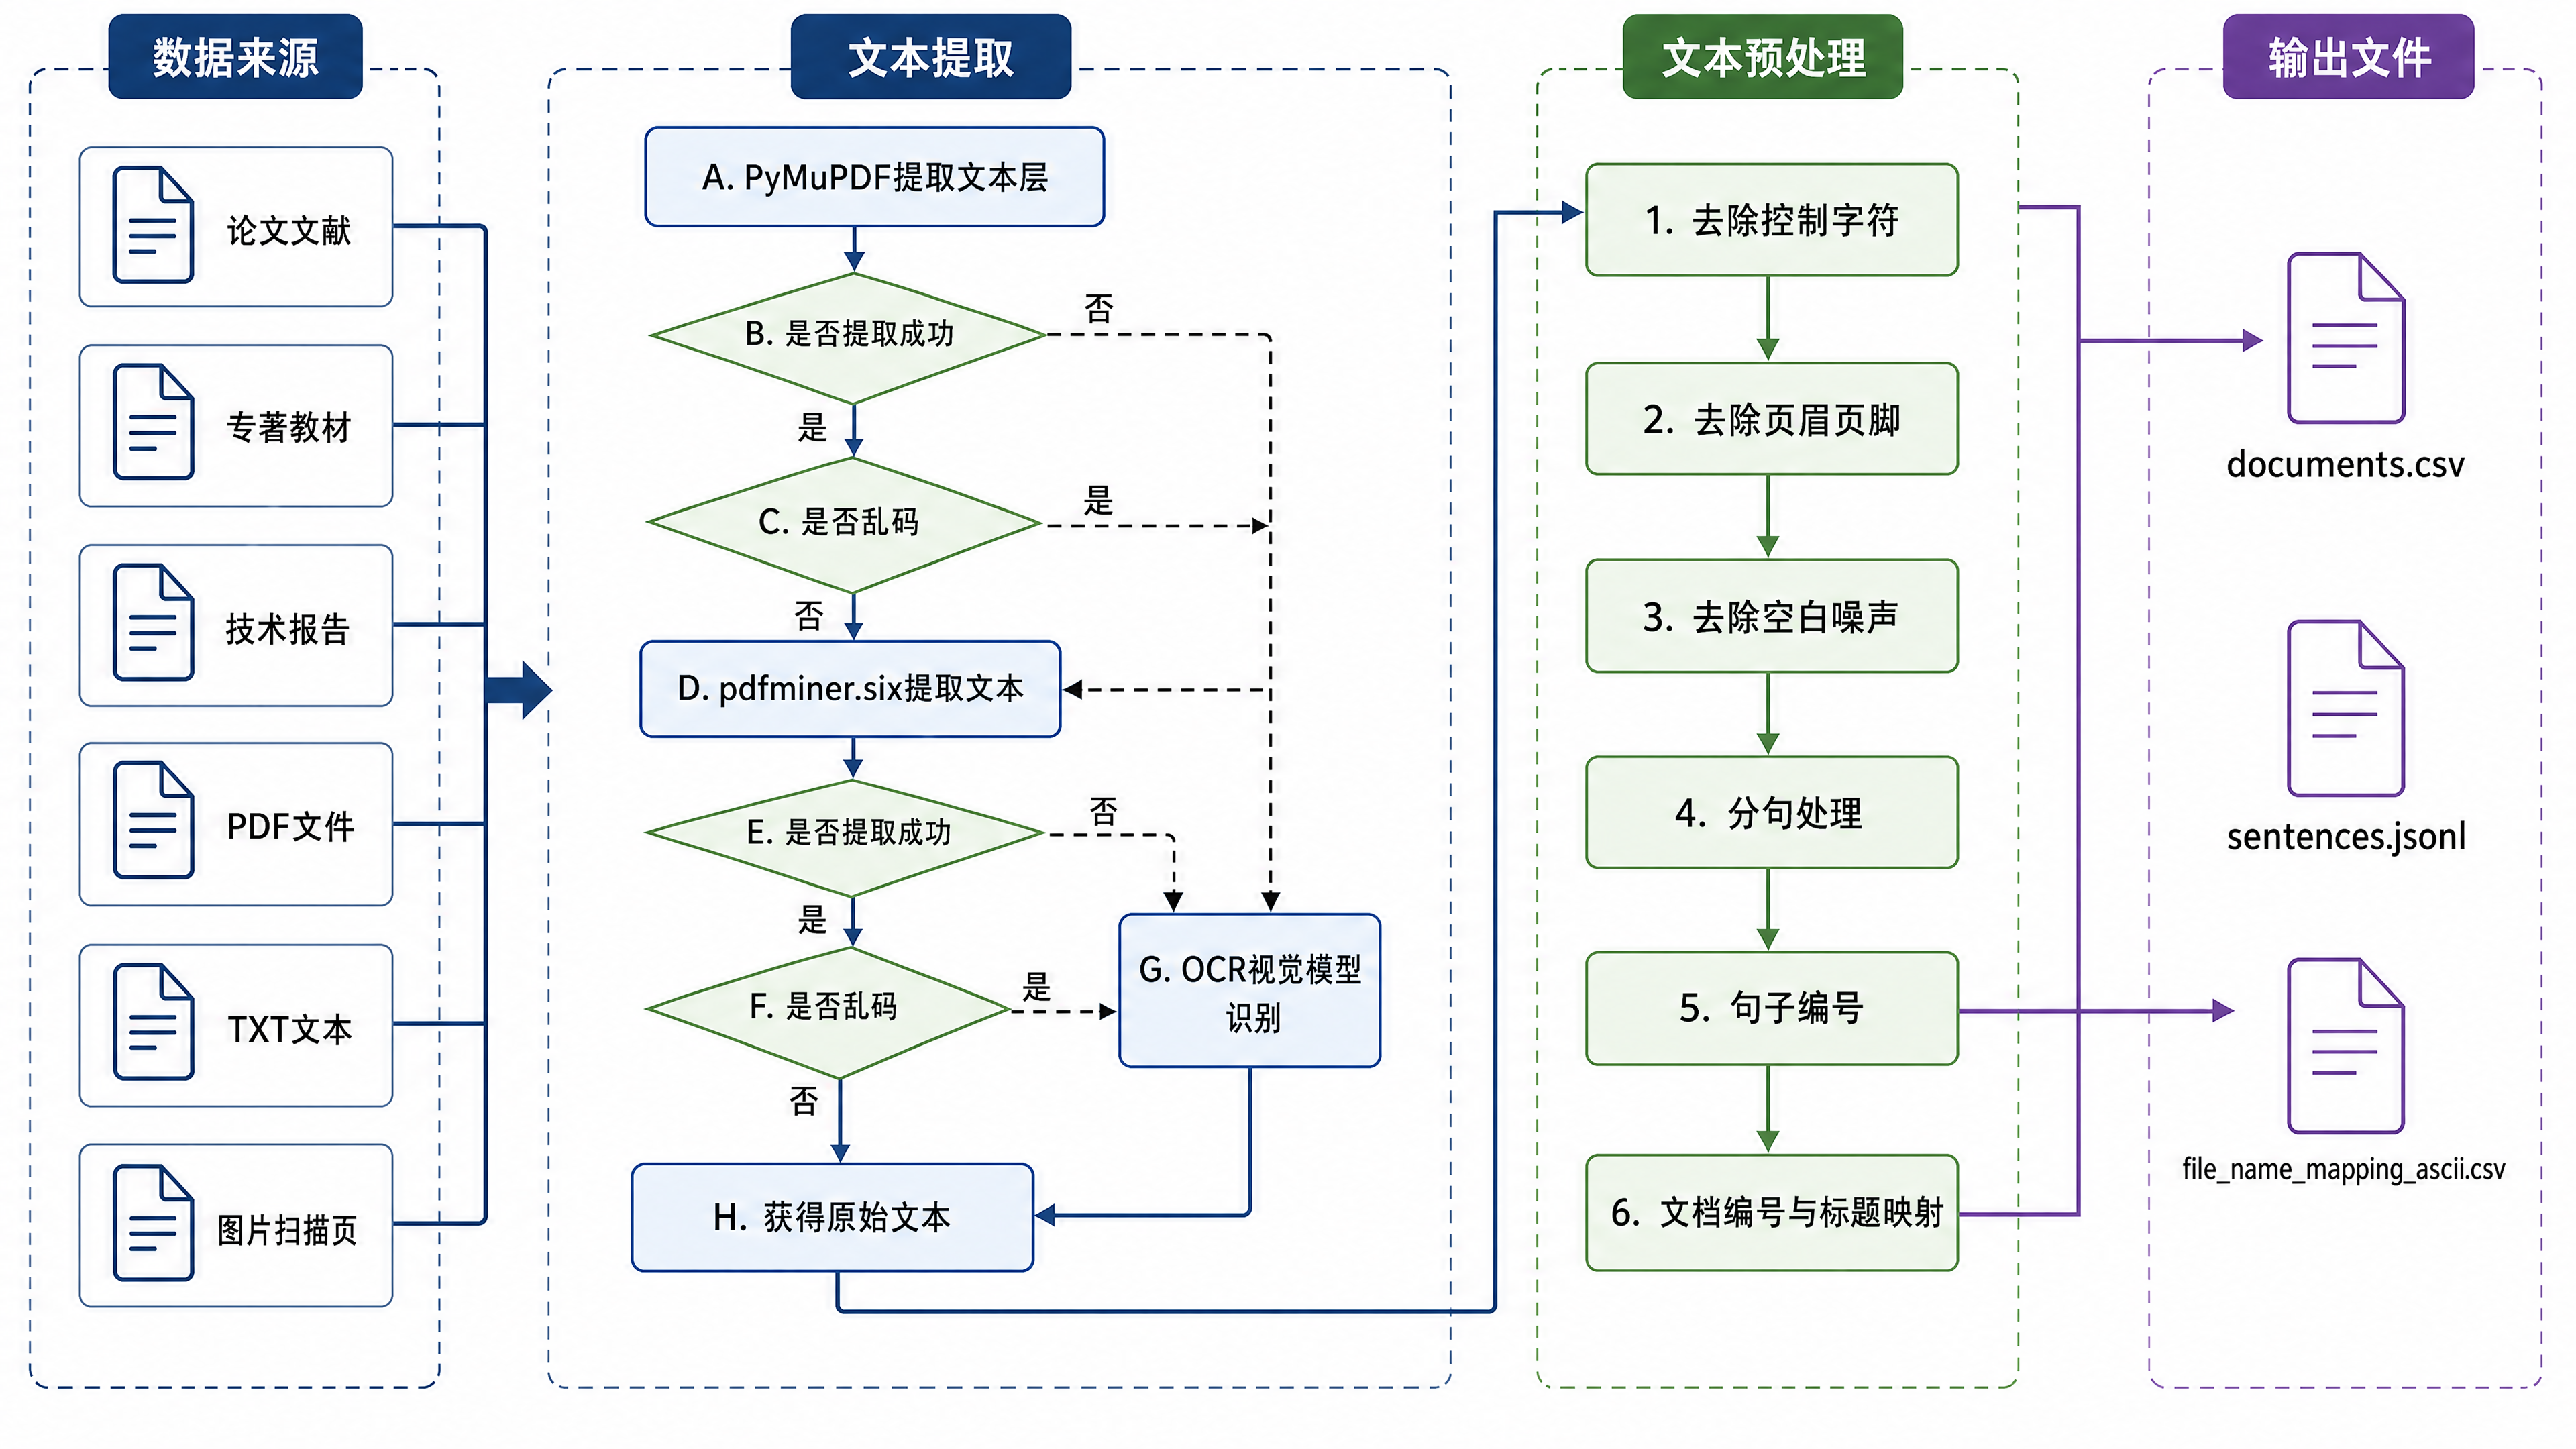
\includegraphics[width=0.88\textwidth]{figures/多源文本提取与预处理流程图.png}
\caption{多源文本提取与预处理流程图}
\label{fig:preprocess}
\end{figure}

\begin{lstlisting}[style=pythonstyle,caption={PDF 文本抽取核心策略示意}]
# preprocess/extract.py
# 1. PyMuPDF 纯文本提取
# 2. pdfminer.six 回退解析
# 3. 视觉模型 OCR 兜底
\end{lstlisting}

\subsubsection{基于术语与规则融合的数据预处理方法}
文本提取完成后，项目继续进行统一换行、去噪、分句和句子编号等处理，将原始文档转化为适合知识抽取的句子级语料。该阶段输出 \texttt{sentences.jsonl}，每条记录包含 \texttt{doc\_id}、\texttt{sentence\_id} 和文本内容，为后续术语统计和实体关系抽取提供标准输入。通过中间结果落盘，系统实现了断点续跑和阶段独立调试，体现了较好的工程规范性。

具体而言，预处理阶段不仅做了基础清洗，还重点处理了影响抽取质量的三类问题：其一是排版噪声，例如页码、重复页眉页脚和跨栏换行造成的句子断裂；其二是结构噪声，例如图题、表题、参考文献段落和公式编号混入正文；其三是语义噪声，例如长度过短且信息量不足的碎片句、过度重复的模板化句子等。通过这一系列处理，系统将面向阅读的文档格式转化为面向算法的可计算语料格式。

如果将原始文档文本序列记作 \(X=\{x_1,x_2,\ldots,x_n\}\)，则预处理函数可写为
\[
S=f_{\mathrm{clean}}(X)=\{s_1,s_2,\ldots,s_m\}
\]
其中 \(S\) 表示最终得到的句子集合。后续的术语抽取、实体识别与关系抽取均在集合 \(S\) 上进行，而不再直接依赖原始排版结构。这种“先标准化，再抽取”的策略显著提高了流水线稳定性，也便于评估阶段在句子级别进行结果对齐。

\subsubsection{利用统计方法与大模型实现关键信息抽取}
术语构建阶段是本项目的重要基础。项目在 \texttt{terminology/term\_extraction.py} 中基于 n-gram、词频、TF-IDF 与 PMI 生成候选术语，并通过综合评分进行排序。候选术语得分定义为
\[
\mathrm{Score}(t)=0.6\cdot \mathrm{freq}(t)+0.3\cdot \mathrm{tfidf}(t)+0.1\cdot \max(\mathrm{PMI}(t),0)
\]
其中 \(t\) 为候选术语，词频体现语料覆盖度，TF-IDF 体现区分能力，PMI 体现术语内部搭配紧密度。该阶段以较高召回率保留潜在领域词，然后通过大模型完成术语是否保留、规范名称和实体类型的定稿判断。这种“先统计、后语义精筛”的方式是本项目的重要创新点之一。

为了增强系统的领域泛化能力，我们对大模型的系统 Prompt 进行了拓展，将其适用范围从单一的“航空航天”扩展至“通用机械与工程（含汽车、液压等）”领域，有效避免了非航天专业文献中通用工程术语被错误过滤的问题。此外，系统还实现了基于 LLM 的增量词典融合与审核机制：在多文档并发上传的场景下，系统会自动读取已有的术语金标准，并与新文档抽取的术语进行去重与融合，从根本上解决了多次上传导致旧图谱内容被覆盖的增量构建难题。

\begin{lstlisting}[style=pythonstyle,caption={候选术语生成示意}]
def generate_candidate_terms(tokens, max_ngram=4):
    counter = Counter()
    ...
    return counter
\end{lstlisting}

\subsection{基于规则约束的知识抽取方法}
在获得术语表后，系统进入实体识别与关系抽取阶段。实体识别采用词典最长匹配和规则补充相结合的方法；关系抽取则采用双模混合逻辑：在有标准词典的明确语境下，结合触发词、位置约束、实体距离阈值和类型约束生成三元组以保证极高的可解释性；而在长难句或隐式关联场景下，系统会自动无缝切换至 LLM 抽取模式进行知识拓扑补全。与完全开放的单一黑盒抽取方式相比，本项目的双模设计更加注重结果质量、可解释性和图谱可展示性。


\newpage
\section{实体类型与逻辑关系}
\subsection{领域实体类型设计}
项目共设计 9 类实体类型：\texttt{Aircraft}、\texttt{Structure}、\texttt{Mechanism}、\texttt{ControlMethod}、\texttt{Performance}、\texttt{Mission}、\texttt{Parameter}、\texttt{Document} 和 \texttt{Concept}。这些类型覆盖了飞行器平台、结构部件、变形机制、控制方法、性能指标、任务场景、参数变量和文献来源等主要知识维度。

\begin{figure}[H]\centering
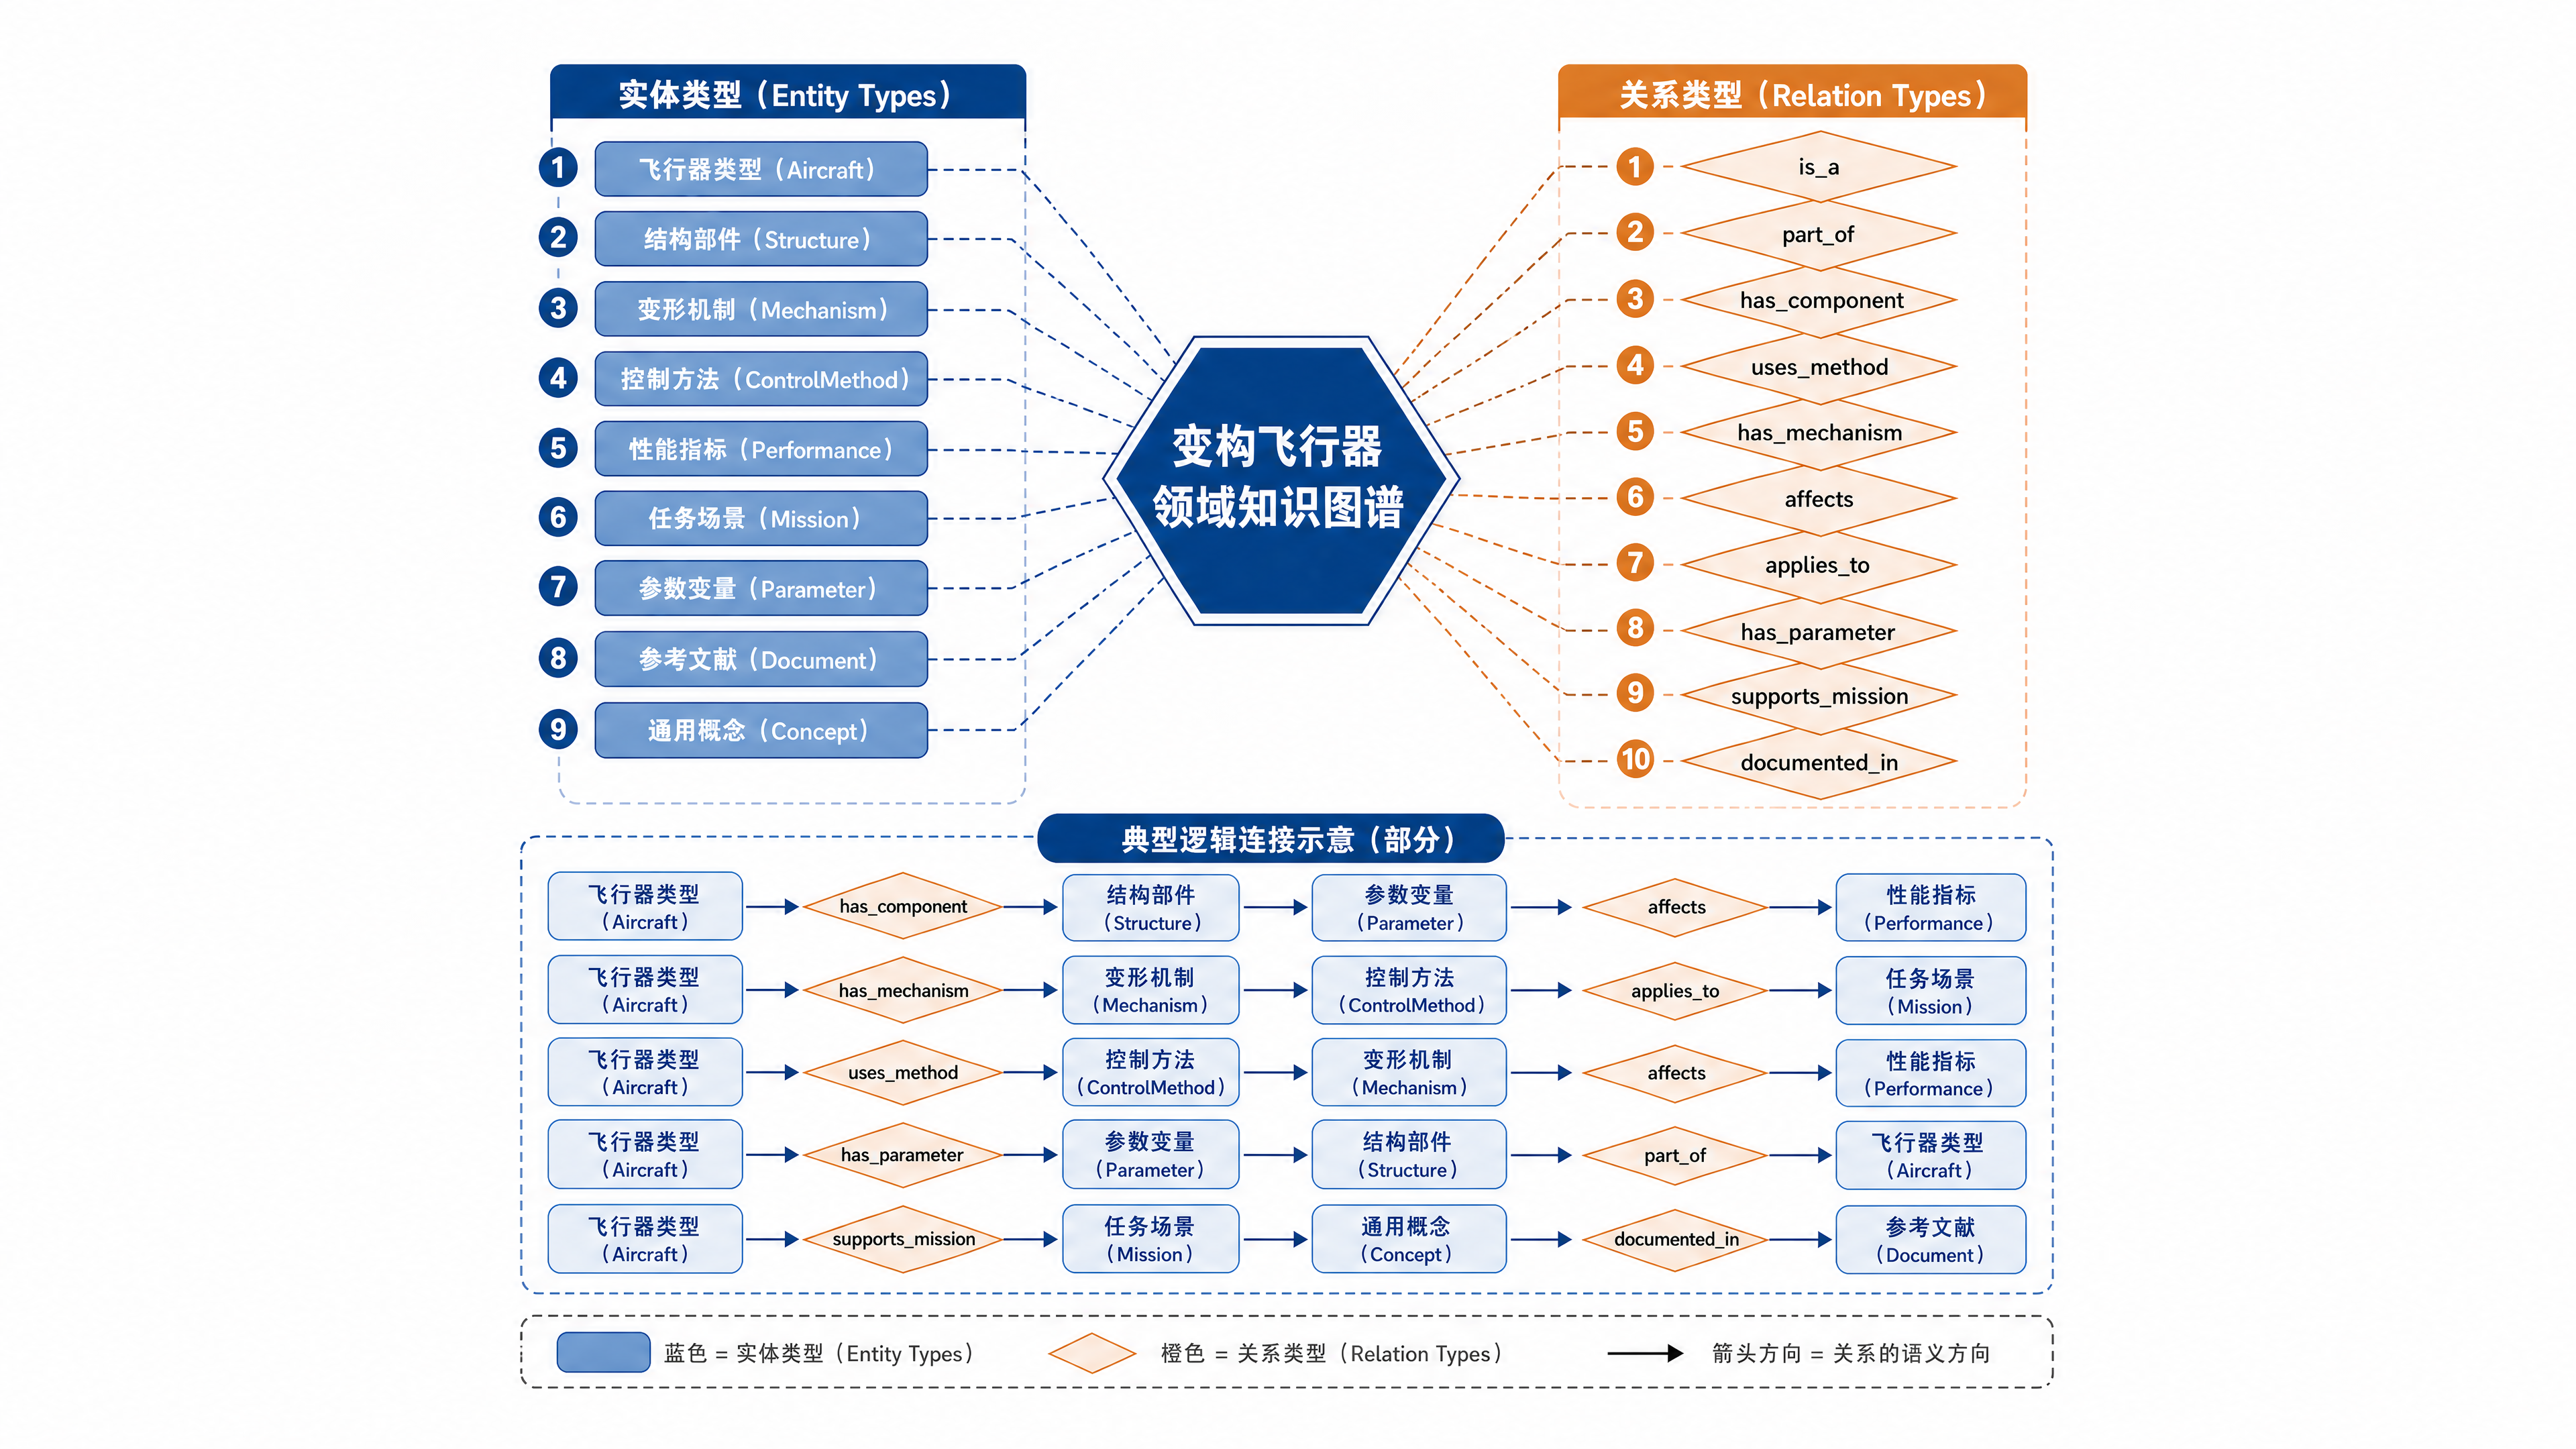
\includegraphics[width=0.85\textwidth]{figures/实体类型与关系类型本体结构图.png}
\caption{实体类型与关系类型本体结构图}
\end{figure}

\begin{figure}[H]\centering
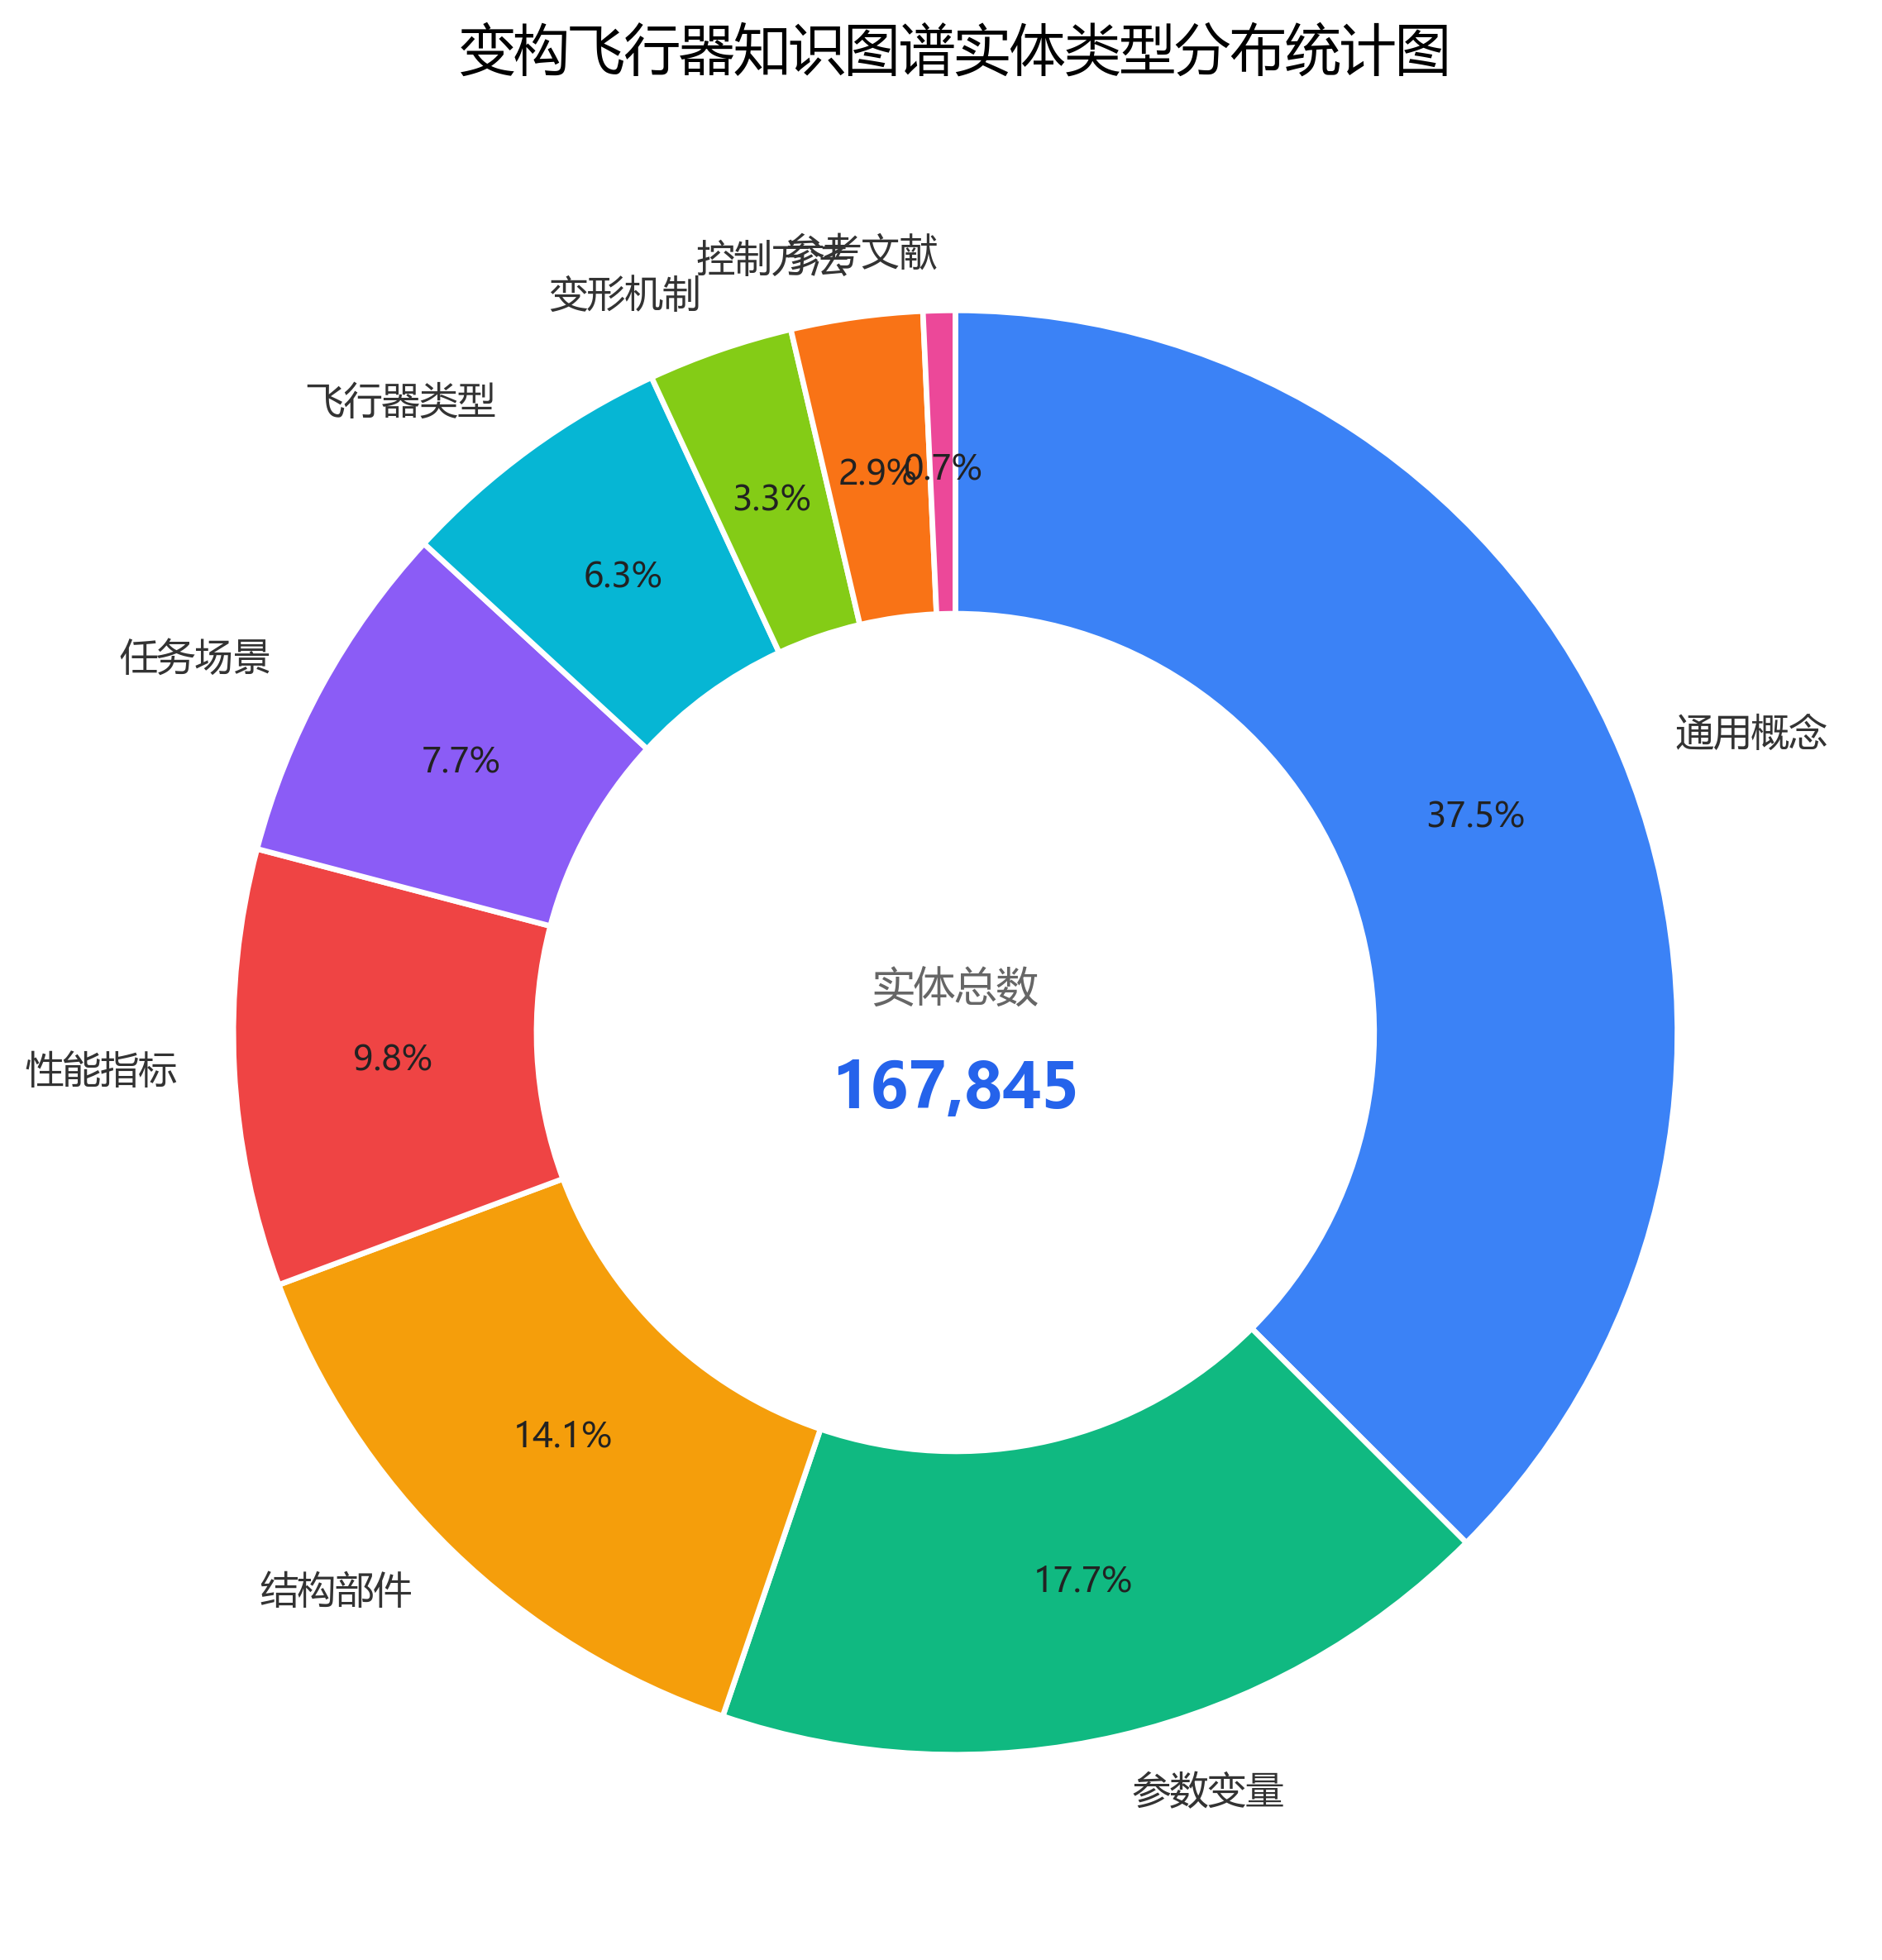
\includegraphics[width=0.5\textwidth]{figures/实体类型分布统计图.png}
\caption{实体类型分布统计图}
\end{figure}

从统计结果看，\texttt{Concept}、\texttt{Parameter} 和 \texttt{Structure} 类型占比最高，说明图谱同时覆盖了大量通用概念、参数知识和结构知识。这与变构飞行器领域“概念体系复杂、结构设计突出、参数分析频繁”的学科特点一致。实体类型体系不仅服务于分类统计，也为后续关系抽取约束提供语义边界。

\subsection{关系类型设计与语义约束}
项目共设计 10 类关系，其中最终结果中主要出现 \texttt{is\_a}、\texttt{has\_component}、\texttt{part\_of}、\texttt{affects}、\texttt{uses\_method}、\texttt{has\_mechanism}、\texttt{supports\_mission}、\texttt{applies\_to} 和 \texttt{has\_parameter}。这些关系覆盖概念层级、结构组成、方法使用、参数影响和任务适用等多种逻辑模式。

\begin{figure}[H]\centering
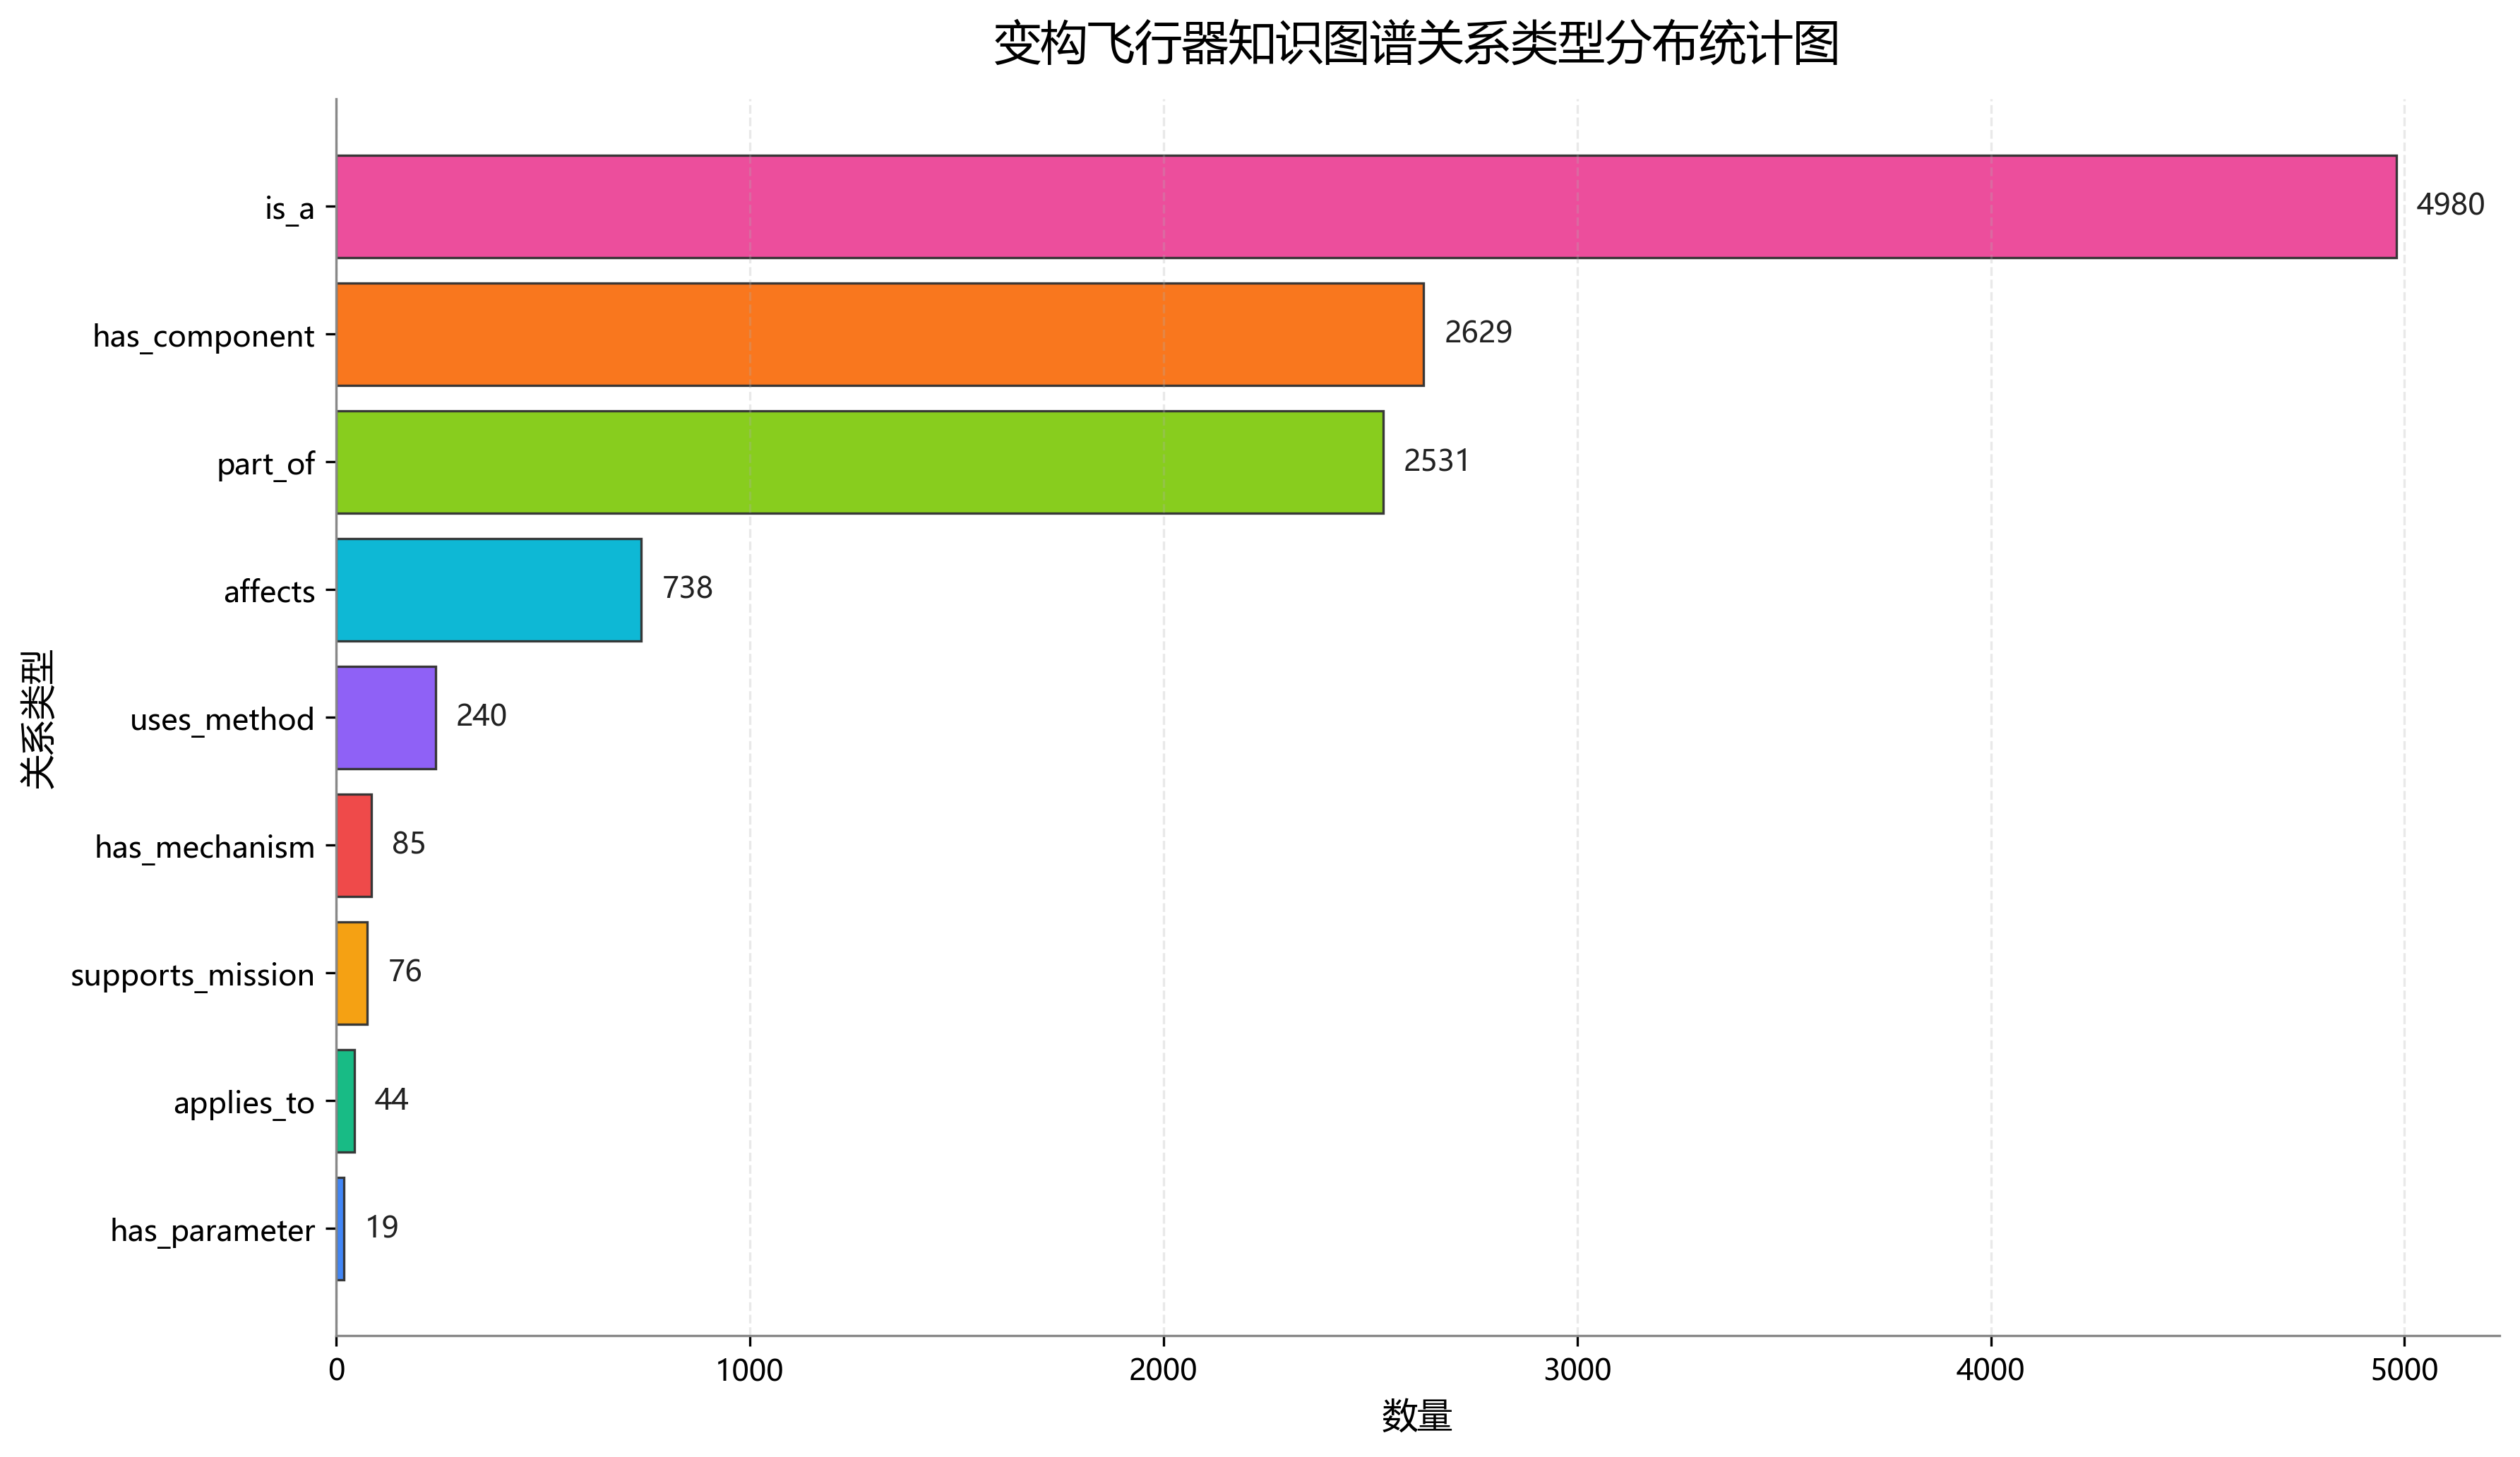
\includegraphics[width=0.82\textwidth]{figures/关系类型分布统计图.png}
\caption{关系类型分布统计图}
\end{figure}

统计结果表明，\texttt{is\_a}、\texttt{has\_component} 和 \texttt{part\_of} 是图谱中占比最高的三类关系，这说明当前图谱在概念层次和组成关系方面最为密集。若记关系为 \(r\)，头尾实体类型分别为 \(h_t\) 与 \(t_t\)，则合法关系可抽象表示为
\[
\mathcal{I}(r,h_t,t_t)=1 \iff (h_t,t_t)\in \Omega_r
\]
其中 \(\Omega_r\) 为关系 \(r\) 的允许类型组合集合。通过这种类型约束，系统有效降低了不合理三元组数量。

\subsection{术语归一化与别名映射机制}
由于领域文献中存在中文全称、英文缩写、修饰性短语等多种表达，项目在术语定稿阶段构建了规范名称与别名映射机制。设原始表达为 \(a\)，规范概念为 \(c\)，则归一化过程可表示为 \(\phi(a)=c\)。这一机制可显著减少图谱中的重复节点，提高搜索和关系聚合效果，也是前端展示稳定性的关键基础。


\newpage
\section{知识图谱构建与系统实现}
\subsection{知识图谱总体架构设计}
项目总体架构包括数据层、预处理层、术语层、抽取层、图谱层、服务层和展示层。数据层负责文献与中间结果管理；预处理层负责文本清洗与分句；术语层负责候选术语生成和 LLM 定稿；抽取层负责实体关系抽取；图谱层负责节点、边和多格式导出；服务层通过 FastAPI 提供接口；展示层基于 ECharts 进行交互可视化。

从实现思想上看，该架构并不是简单的脚本堆叠，而是典型的流水线式工程组织。每一层都以标准化文件作为输入输出边界：例如预处理层输出句子级语料，术语层输出定稿术语表，抽取层输出实体与关系记录，图谱层输出节点和边集合。这种层次化拆分使得系统具备良好的可维护性与可复现实验能力。若某一阶段策略发生变化，如术语筛选阈值调整或关系触发词补充，仅需重跑局部阶段即可，无需完全从头执行全部流程。

同时，该架构兼顾了课程项目场景下的展示需求与技术扩展性。一方面，当前系统可直接依赖本地文件运行，无需预先搭建复杂数据库环境，降低了部署门槛；另一方面，图谱层保留 JSON、CSV 与 TTL 等标准导出格式，为后续接入图数据库、RDF 推理框架或问答系统提供了接口基础。因此，这一总体架构既满足了原型系统快速实现的现实要求，也为未来扩展留出了清晰空间。

\subsection{实体抽取与关系抽取实现}
实体识别以 \texttt{terms\_final.csv} 为词典基础，辅以规则识别部分参数类与结构类实体。关系抽取则采用“同句实体对—触发词匹配—约束过滤—三元组输出”的流程。项目引入触发词位置约束、实体黑名单、距离阈值和实体类型约束四重过滤机制，显著提高了关系抽取的精度。

在实体抽取阶段，系统重点解决的是“高召回识别”与“实体边界稳定”之间的平衡问题。若词典过小，则容易遗漏大量领域术语；若词典过大，则容易引入噪声概念。因此项目先通过术语构建阶段尽量扩大候选覆盖，再在抽取阶段通过最长匹配、重叠消解和类型校验抑制误识别。例如，较长的专业术语在匹配时具有更高优先级，以避免短词将长词切碎；同时，对明显缺乏领域意义的黑名单词项进行过滤，以减少通用词误判为实体的现象。

在关系抽取阶段，系统强调“可解释规则优先”与“大语言模型增强”相结合的双模理念。对于具有金标准的明确术语，系统通过显式触发词模式定义候选关系类型，再结合实体类型兼容性、实体间最大距离和句内位置顺序进行过滤，保证抽取的高度可解释性。为了弥补纯规则抽取带来的图谱稀疏（“散点图”）问题，系统在降级模式下引入了基于大模型的上下文感知三元组抽取。该模块将包含多个候选实体的长难句进行动态批处理（每批约 200 条），并通过 \texttt{ThreadPoolExecutor} 开启多达 8 个并发工作线程。这种并行计算架构不仅大幅缩短了处理耗时，更凭借 LLM 的语义理解能力有效覆盖了规则难以处理的隐式关联。

\begin{figure}[H]\centering
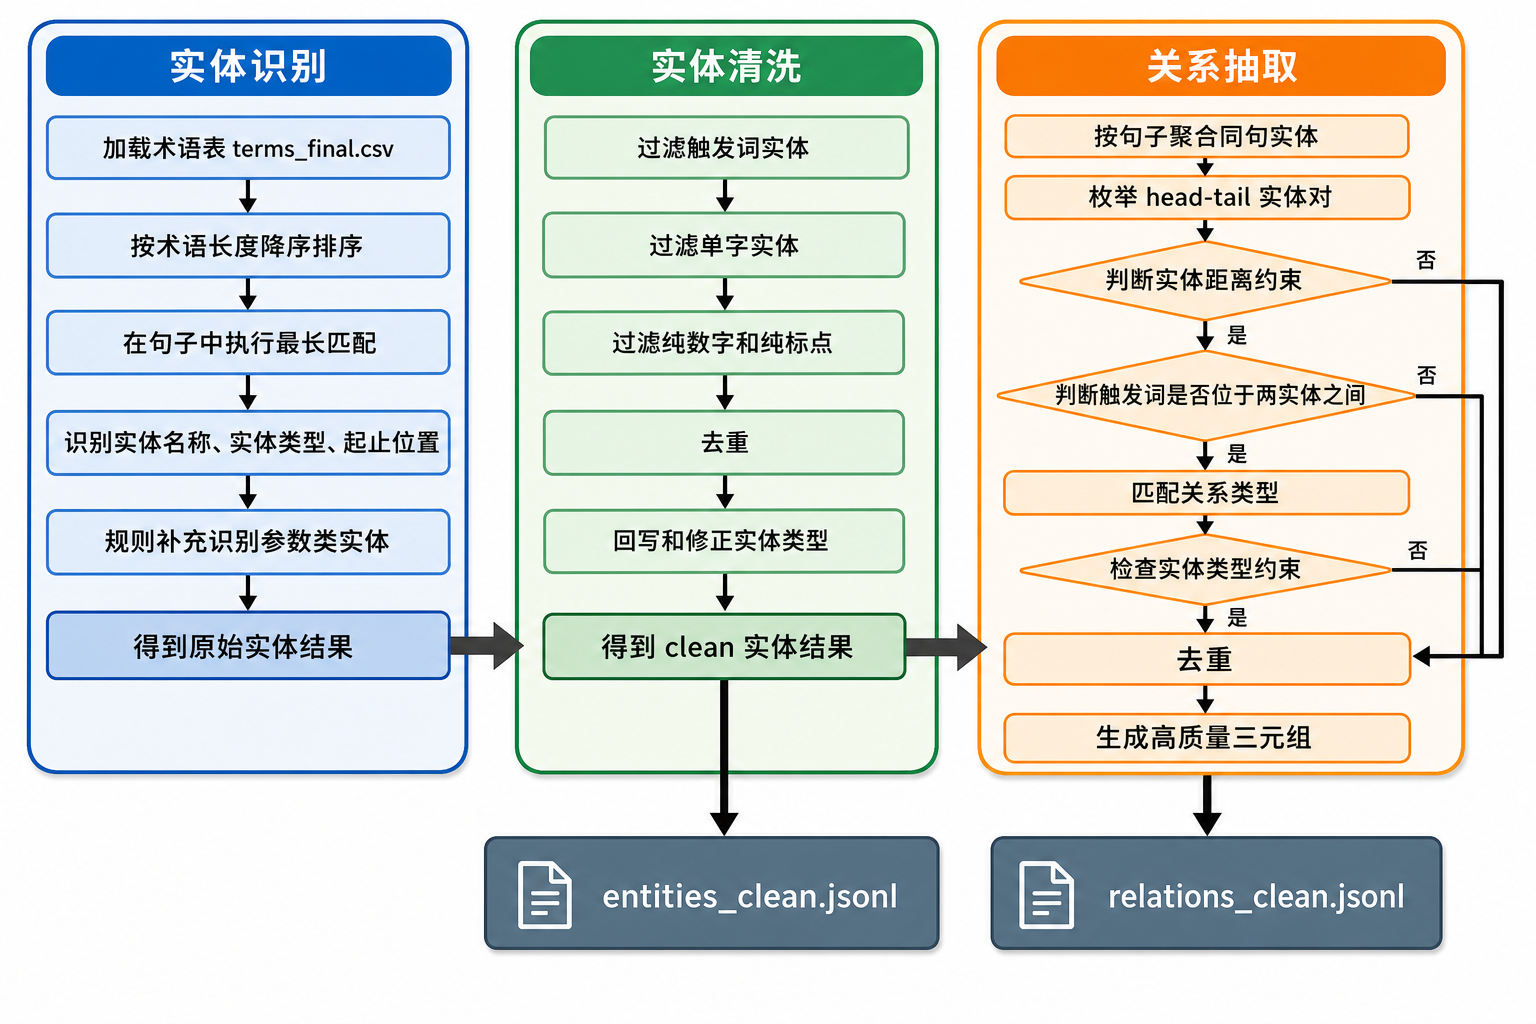
\includegraphics[width=1\textwidth]{figures/实体识别与关系抽取流程图.png}
\caption{实体识别与关系抽取流程图}
\end{figure}

\begin{lstlisting}[style=pythonstyle,caption={关系抽取约束示意}]
RELATION_PATTERNS = [
    ("is_a", ["是一种", "属于", "可视为"]),
    ("has_component", ["包括", "包含", "组成"]),
]
MAX_ENTITY_DISTANCE = 80
\end{lstlisting}

\subsection{图谱数据导出与存储}
图谱构建模块将实体与关系组织为节点集和边集，并导出为 \texttt{kg.json}、\texttt{nodes.csv}、\texttt{edges.csv} 和 \texttt{kg.ttl}。其中 \texttt{kg.json} 直接供前端使用，CSV 便于图数据库导入，TTL 便于 RDF 语义表达。这样的多格式导出方式体现了较强的规范性和扩展性。

在导出阶段，系统并不是简单地将抽取结果原样写出，而是先进行节点去重、名称标准化和关系重组，再根据不同使用场景输出不同格式的数据文件。图~\ref{fig:export} 展示了这一过程，有助于说明图谱结果如何从抽取记录转化为可展示、可分析、可复用的结构化图谱数据。

\begin{figure}[H]\centering
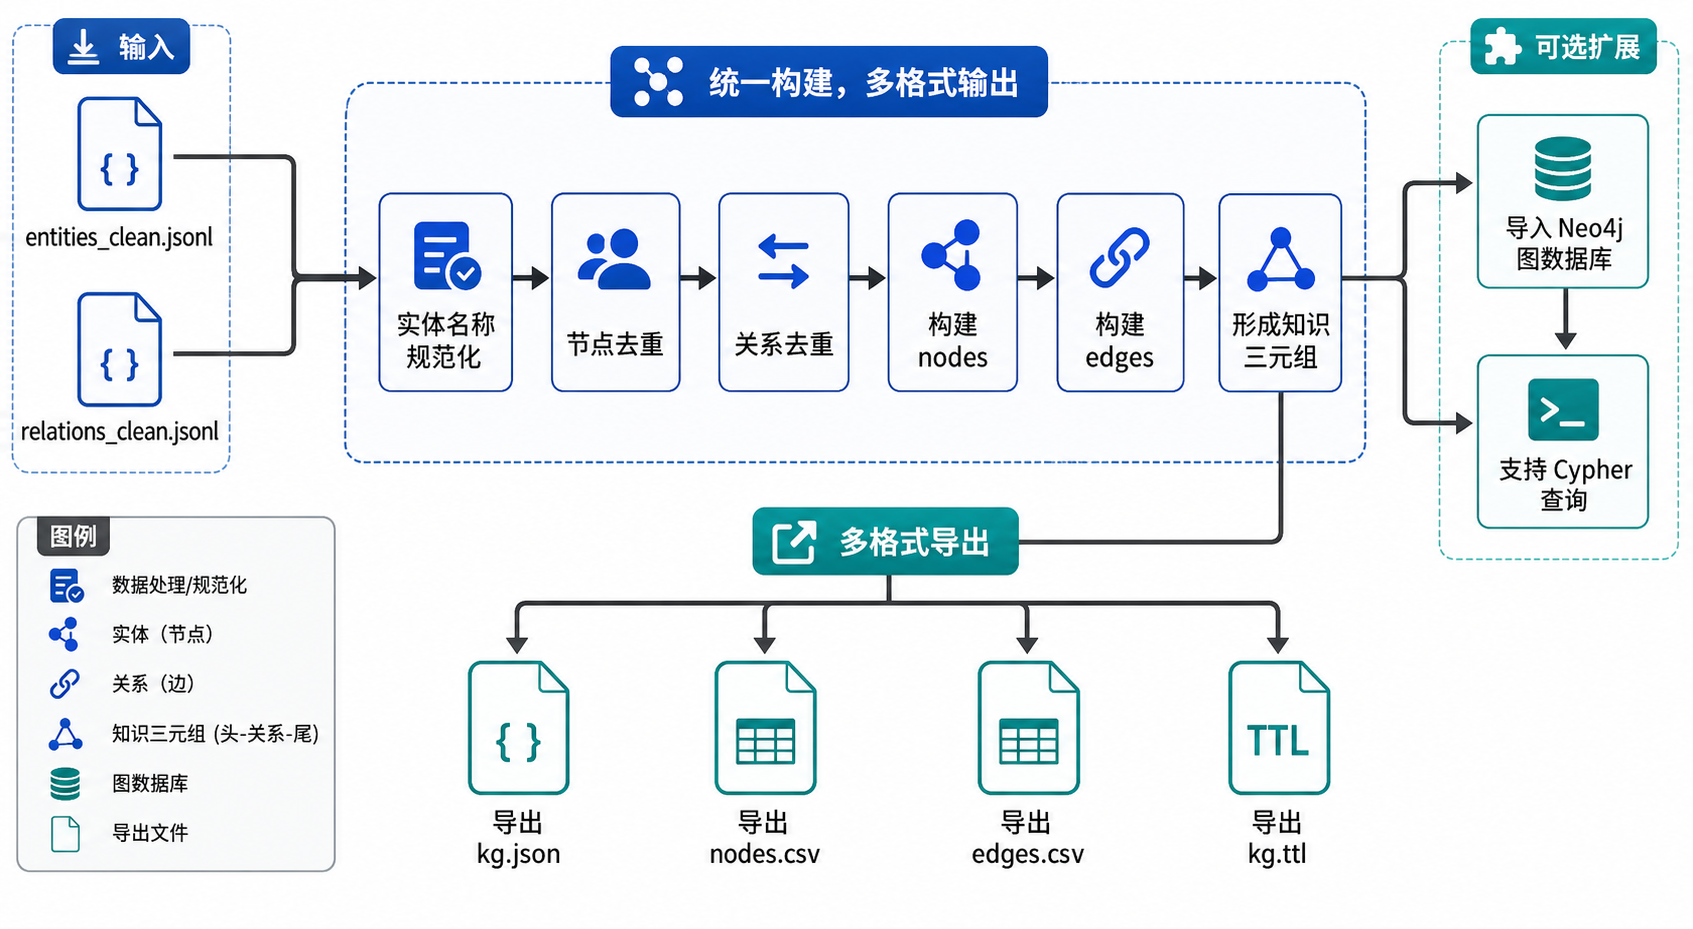
\includegraphics[width=0.86\textwidth]{figures/知识图谱构建与多格式导出流程图.png}
\caption{知识图谱构建与多格式导出流程图}
\label{fig:export}
\end{figure}

\subsection{知识图谱可视化系统实现}
项目使用 FastAPI + ECharts 构建了轻量级前后端一体化图谱系统。后端直接加载 \texttt{kg.json} 即可运行，避免了答辩环境中必须部署图数据库的复杂性；前端支持图谱总览、实体搜索、类型筛选、实体详情展示与局部子图钻取，使图谱不仅可以被看到，还可以被解释和分析。

在后端实现上，系统将图谱统计、搜索、节点详情和中心子图等功能封装为独立接口，从而使前端页面逻辑与底层数据组织方式解耦。这样做的好处在于：一方面可以让前端专注于交互与展示，另一方面也便于后续将文件型图谱替换为数据库型图谱而不必完全重写前端逻辑。在前端实现上，力导向图被用作主要展示形式，是因为它更适合呈现实体之间的聚类关系、中心节点和局部连接强度，有助于用户从视觉上快速把握图谱结构。

此外，系统在可视化层面并非仅追求“好看”，而是尽量服务于知识探索任务。实体搜索帮助用户快速定位目标概念；类型筛选帮助用户隔离不同语义层次的节点；实体详情面板帮助用户查看节点属性与关联边；局部子图则帮助用户以某个中心实体为起点展开邻域分析。在交互体验优化方面，前端重构了关键操作的确认逻辑，通过自定义异步 Modal 对话框替换了原生 \texttt{window.confirm}，彻底解决了大规模并行构建任务中浏览器 UI 线程被阻塞的缺陷。通过这些功能，图谱由静态结果图转化为流畅可交互的知识组织界面，这也是本项目的重要实现特点之一。

图~\ref{fig:main-ui} 展示了系统主界面。该界面主要用于呈现知识图谱整体分布、节点聚类状态以及全局交互效果，是用户进入系统后最先接触到的总览页面。通过主界面，用户可以先形成对图谱规模、结构和热点实体的整体认识，再进一步进行局部探索。

\begin{figure}[H]\centering
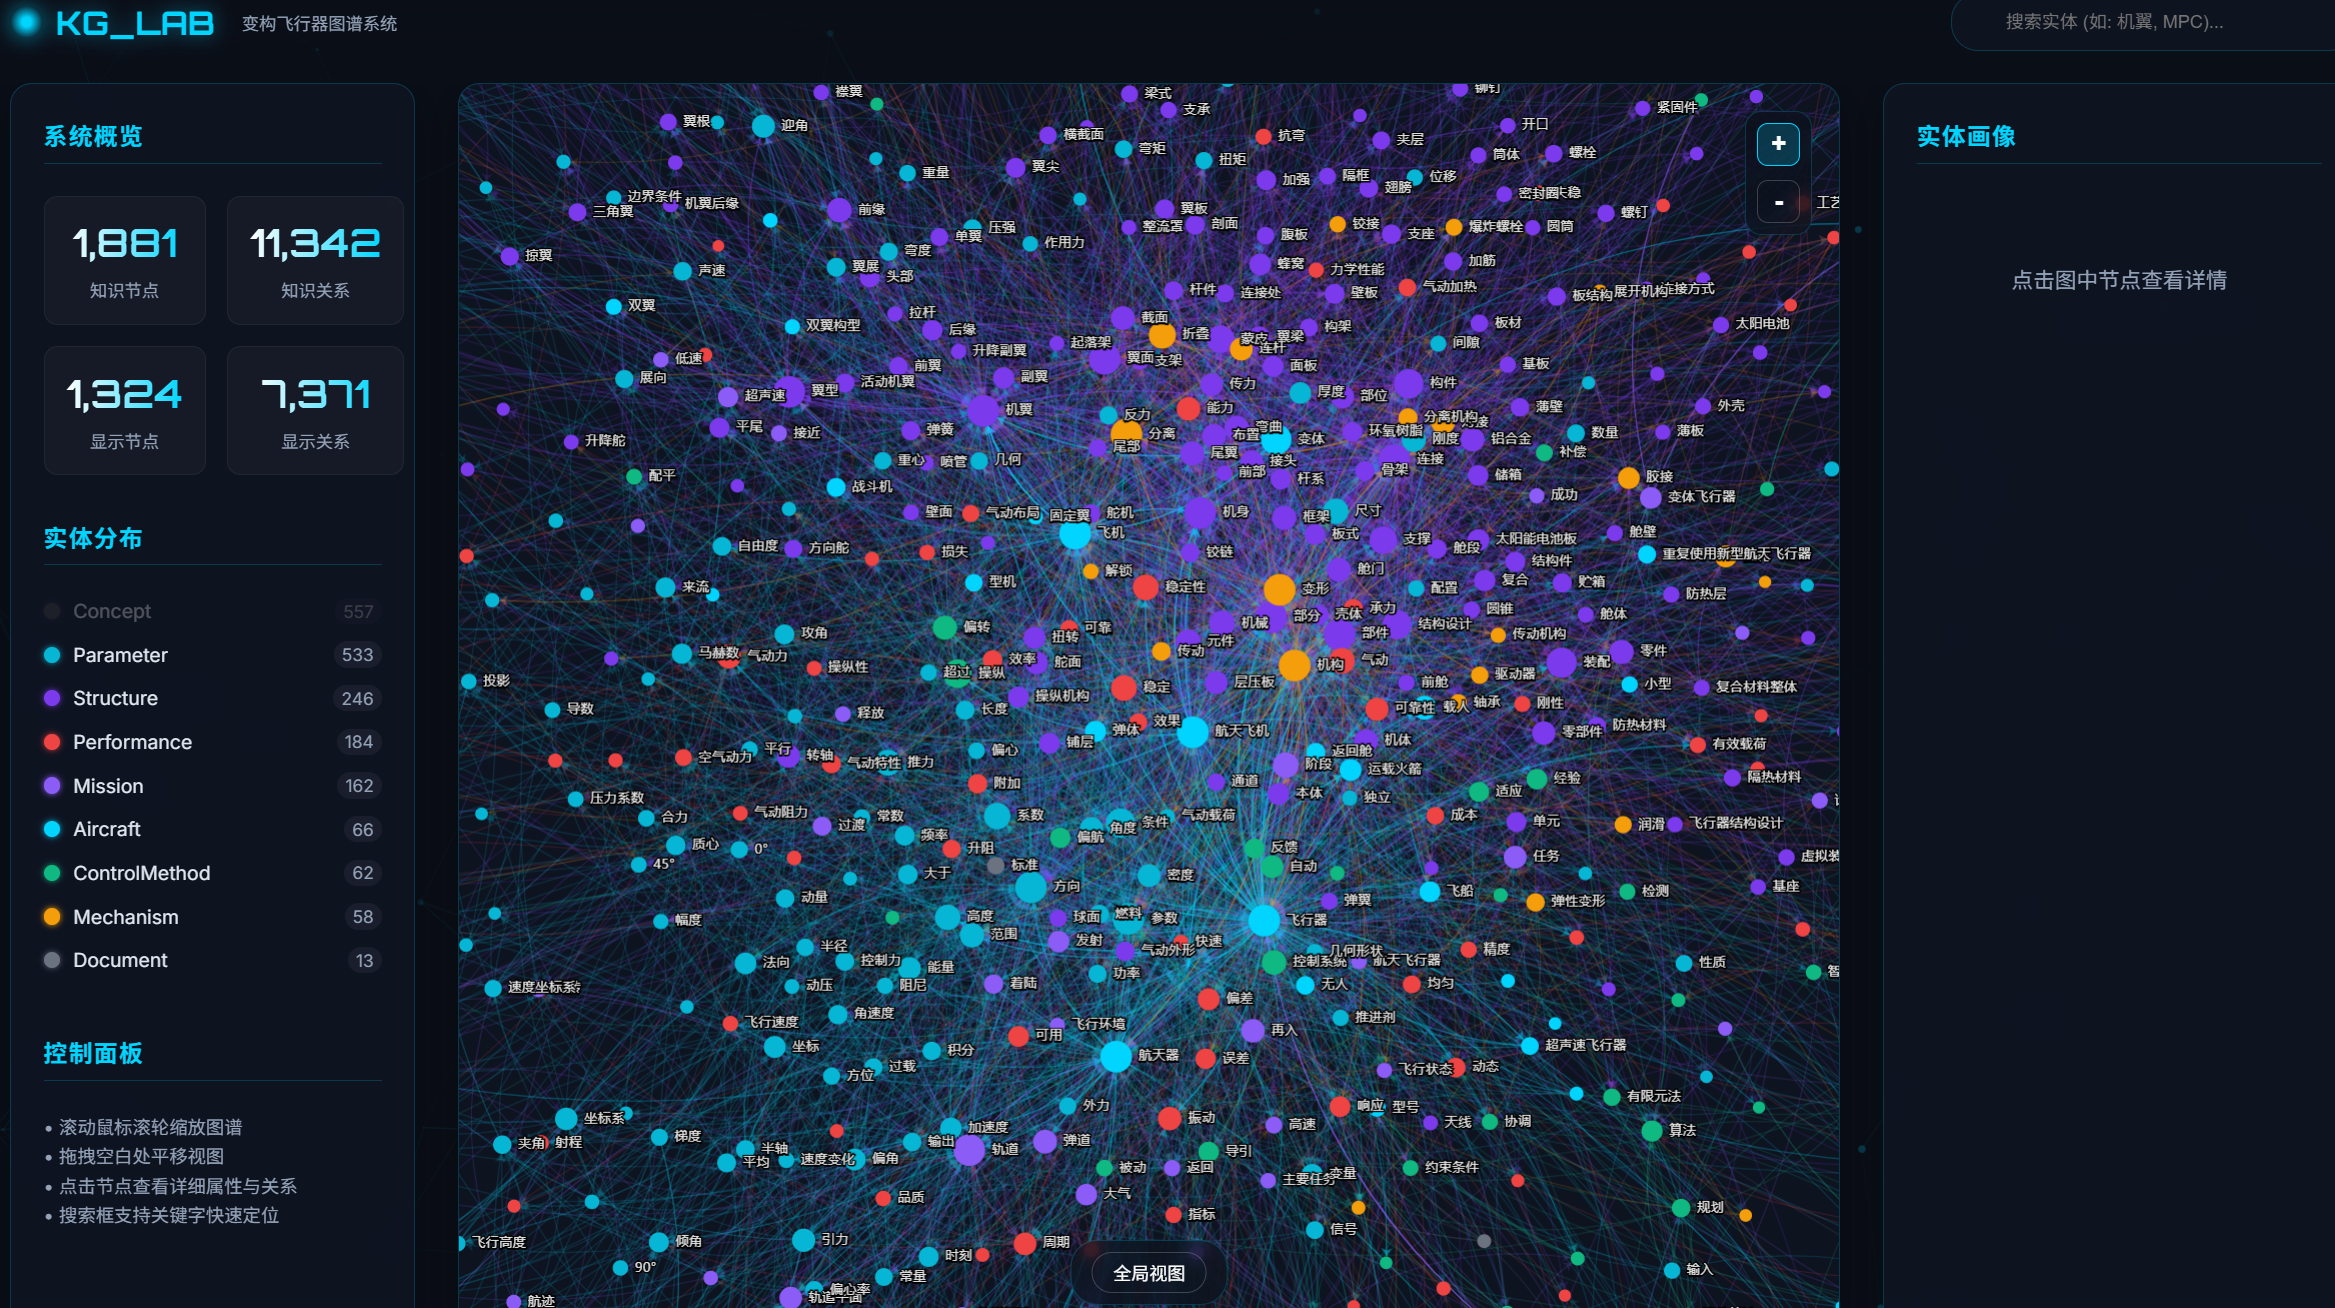
\includegraphics[width=0.90\textwidth]{figures/前端整体展示图.png}
\caption{知识图谱可视化系统主界面}
\label{fig:main-ui}
\end{figure}

在完成整体浏览后，用户还需要查看单个实体的属性信息及其周边关系。图~\ref{fig:detail-ui} 展示了实体详情与关联关系展示界面，该界面能够将中心实体的基本信息、关联节点和对应关系同步呈现，便于分析某一概念在图谱中的语义位置与关联范围。

\begin{figure}[H]\centering
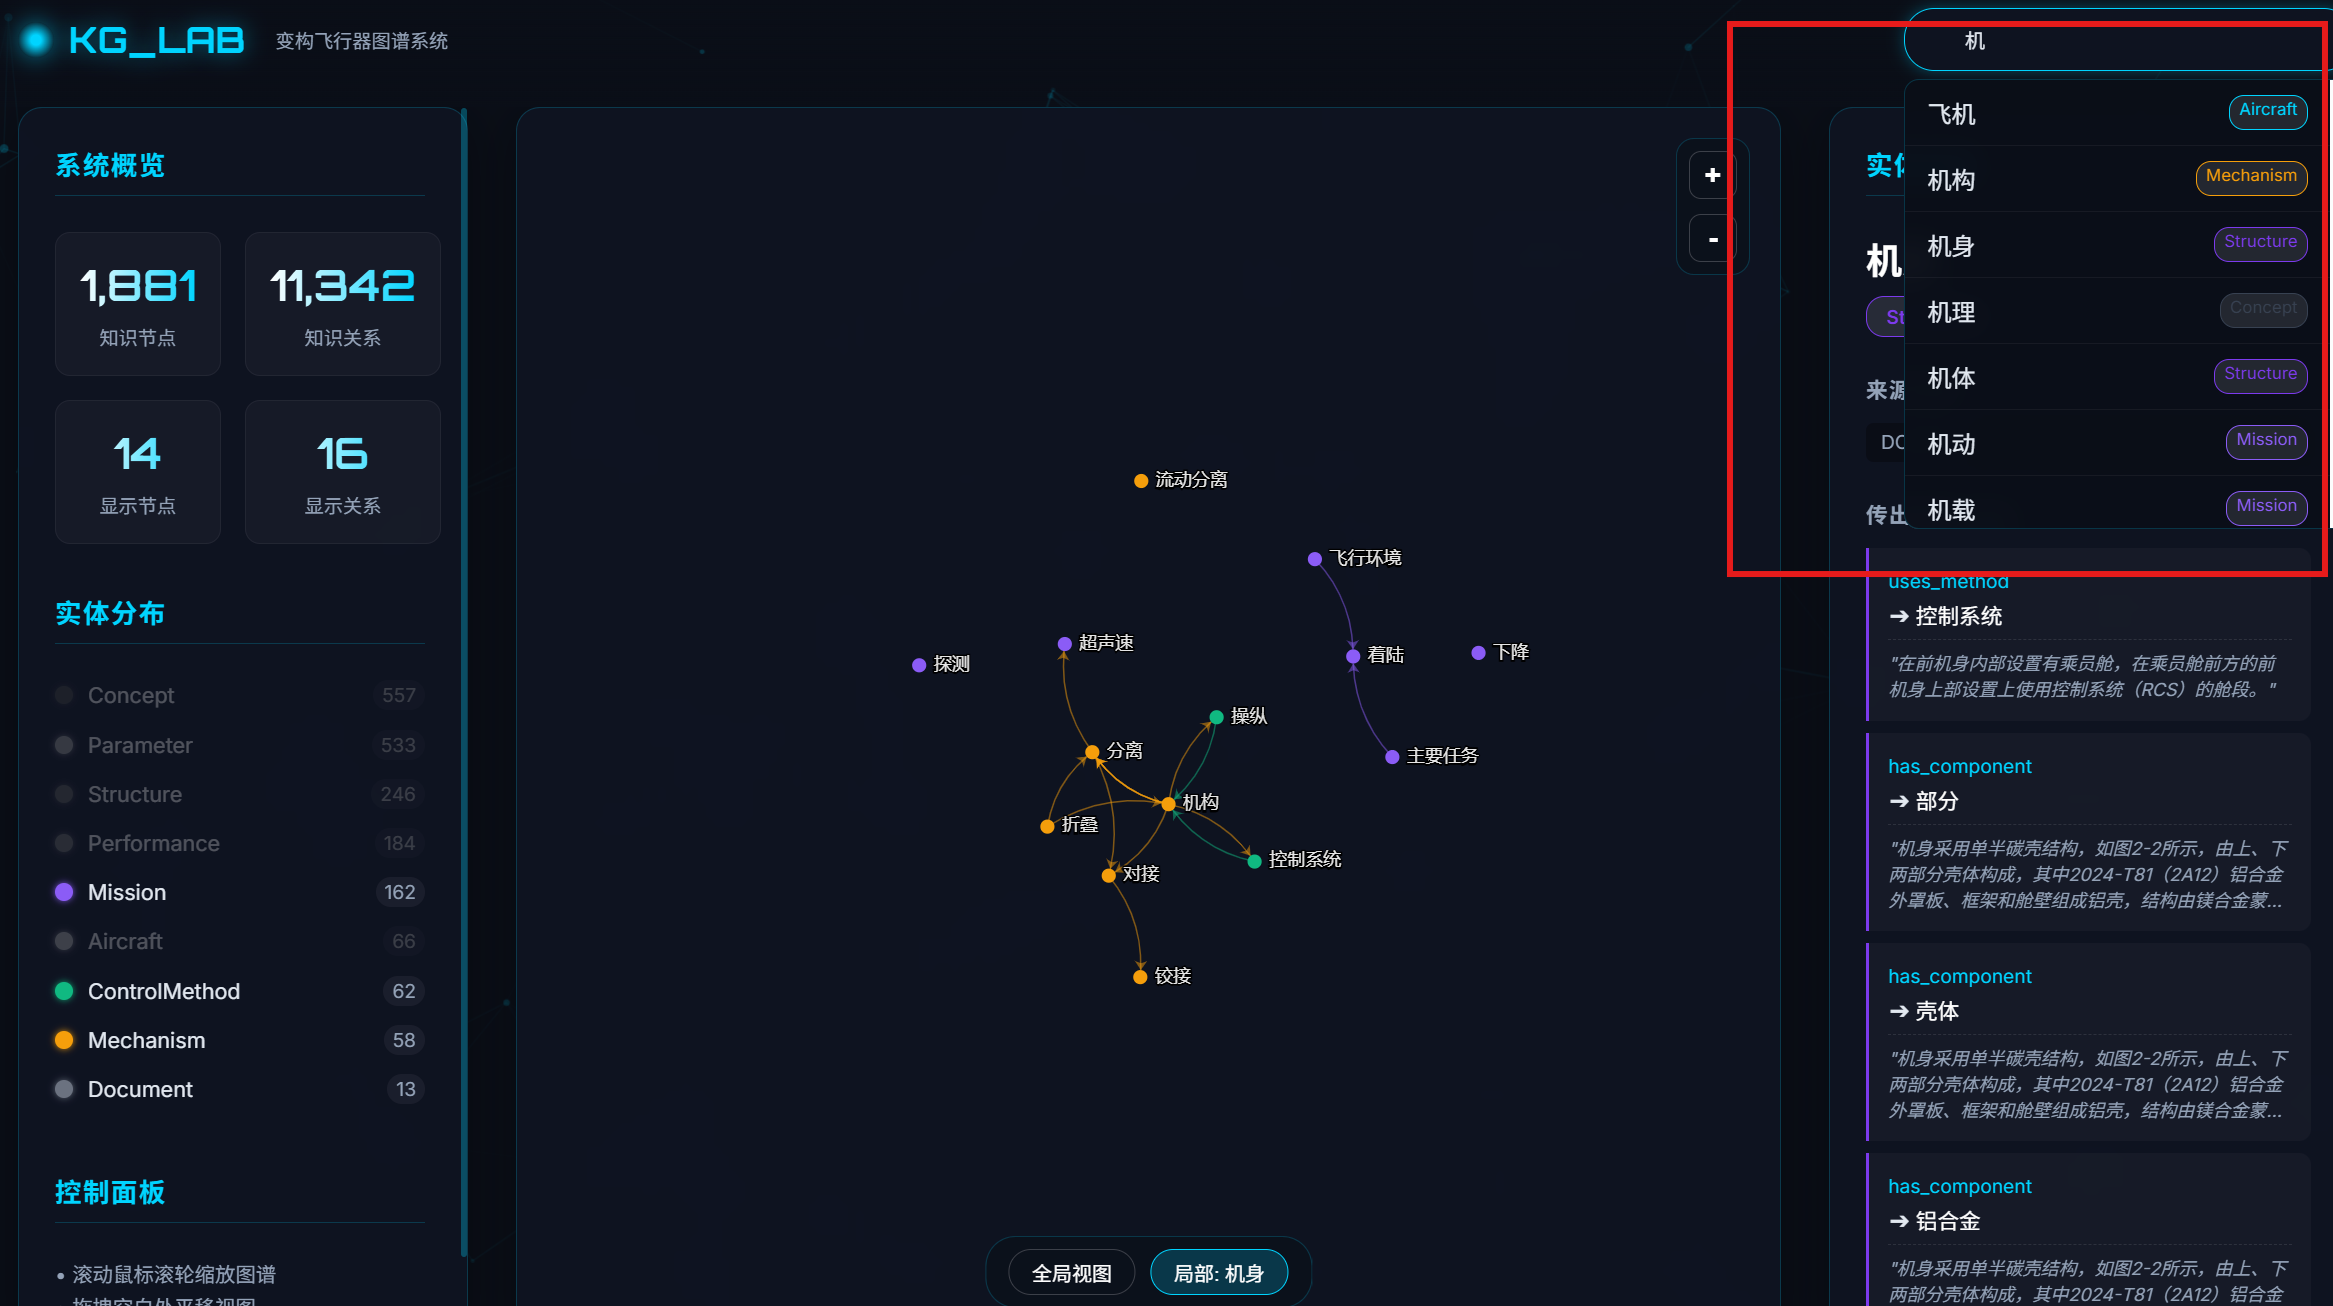
\includegraphics[width=0.9\textwidth]{figures/实体详情与关联关系展示界面.png}
\caption{实体详情与关联关系展示界面}
\label{fig:detail-ui}
\end{figure}

当用户希望从更高层次理解图谱中不同类型实体的分布结构时，类型筛选功能就变得尤为重要。图~\ref{fig:filter-ui} 展示了基于实体类型筛选的图谱显示效果。通过对不同实体类别进行过滤，用户可以更清晰地观察某一类节点的聚合形态及其与其他类型节点之间的连接模式，从而提高图谱分析的针对性。

\begin{figure}[H]\centering
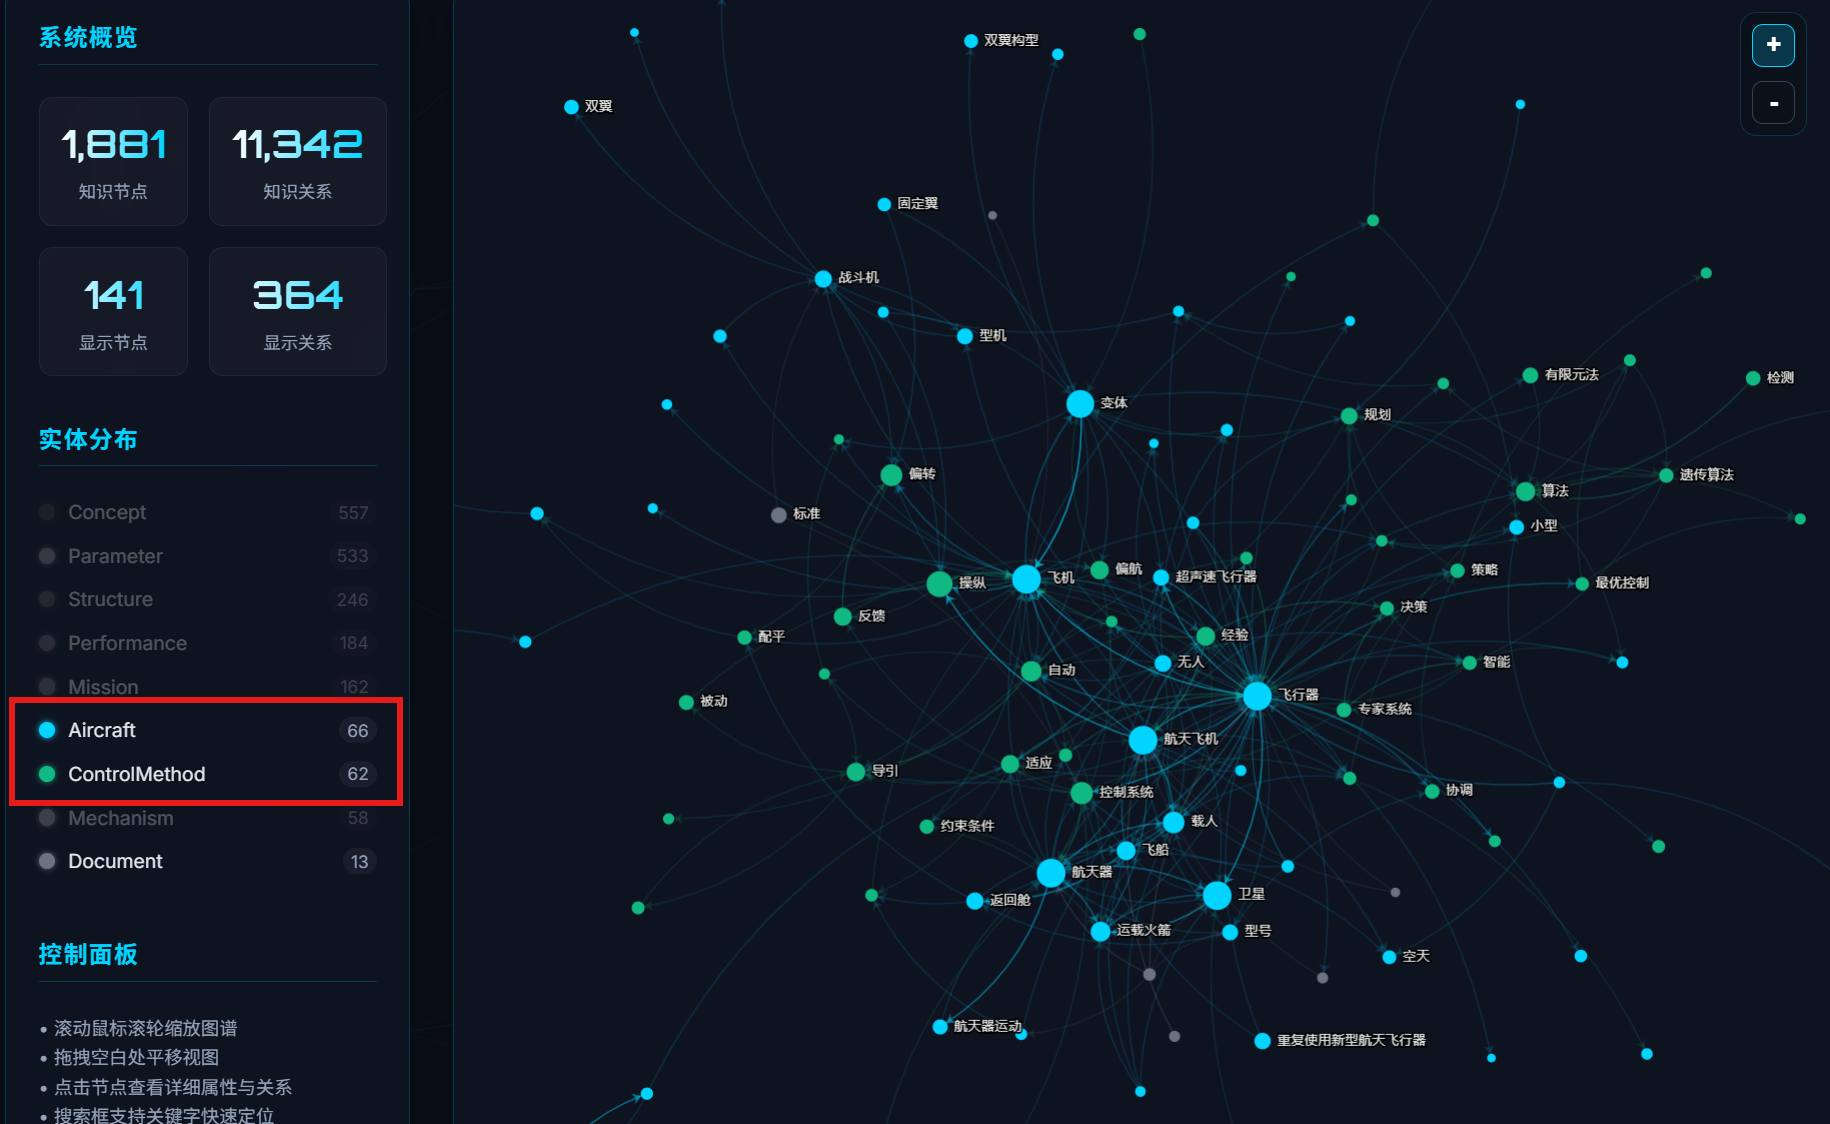
\includegraphics[width=0.9\textwidth]{figures/基于实体类型筛选的图谱显示效果.png}
\caption{基于实体类型筛选的图谱显示效果}
\label{fig:filter-ui}
\end{figure}


\newpage
\section{实验评估与结果分析}
\subsection{评估流程设计}
为了验证抽取效果，项目构建了人工金标准数据，并采用 Precision、Recall 和 F1 作为标准评估指标。若 \(TP\)、\(FP\)、\(FN\) 分别表示真正例、假正例和漏检数，则
\[
P=\frac{TP}{TP+FP},\qquad R=\frac{TP}{TP+FN},\qquad F_1=\frac{2PR}{P+R}
\]
项目在评估脚本中先利用人工标注句子范围过滤预测结果，再进行集合碰撞，从而保证评估逻辑合理。

\begin{figure}[H]\centering
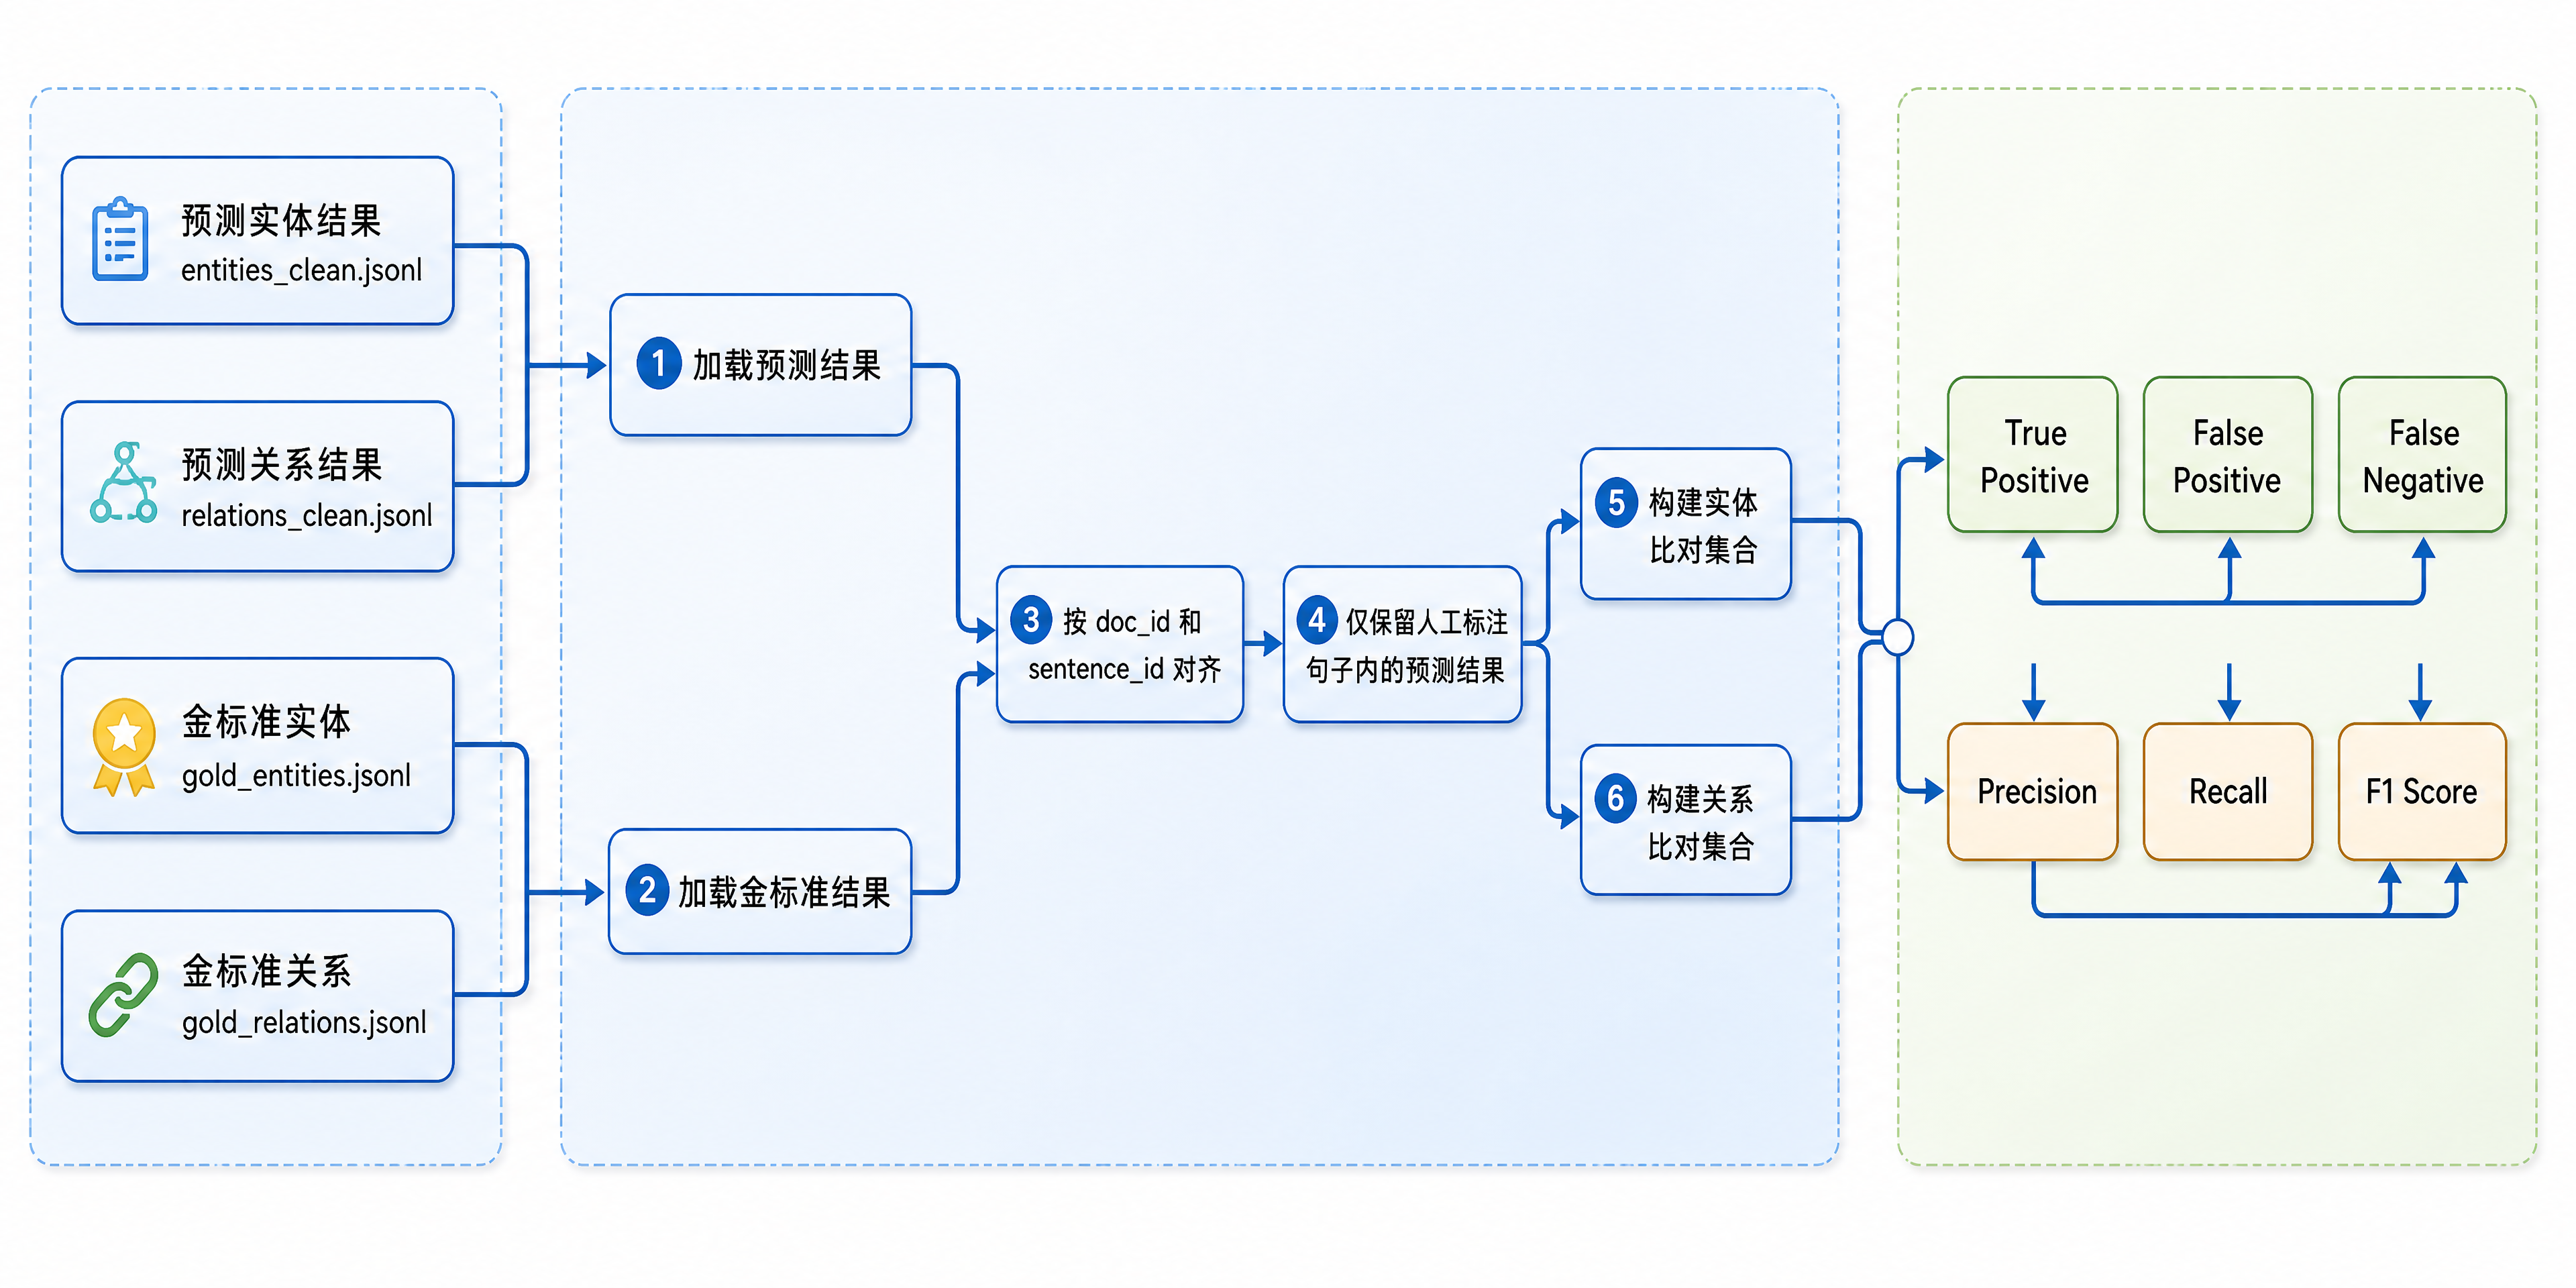
\includegraphics[width=0.88\textwidth]{figures/知识抽取算法评估流程图.png}
\caption{知识抽取算法评估流程图}
\end{figure}

\subsection{结果规模与统计分析}
从结果规模看，项目产生了 167846 条实体记录，并构建出约 1881 个知识节点和 11342 条知识关系。实体分布和关系分布统计表明，当前图谱在概念层次、结构组成和参数性能关联方面具有较好的覆盖度。整体结果说明，本项目已经具备了构建千级节点、万级关系图谱并进行前端可视化展示的能力。

在人工金标准评估中，实体抽取与关系抽取结果如表~\ref{tab:eval-all} 所示。可以看出，本项目在实体抽取任务上取得了较好的综合效果，Precision、Recall 和 F1 分别达到 87.12\%、97.52\% 和 92.03\%；关系抽取任务的 Precision、Recall 和 F1 分别达到 81.68\%、95.34\% 和 87.98\%。从指标分布看，系统整体呈现“召回率高于精确率”的特征，这说明当前方法具有较强的知识覆盖能力，同时仍存在一定的过抽取现象。

\begin{table}[H]
\centering
\caption{实体与关系抽取算法综合评估结果}
\label{tab:eval-all}
\renewcommand{\arraystretch}{1.28}
\resizebox{\textwidth}{!}{%
\begin{tabular}{>{\centering\arraybackslash}p{2.3cm}>{\centering\arraybackslash}p{2.1cm}>{\centering\arraybackslash}p{2.4cm}>{\centering\arraybackslash}p{2cm}>{\centering\arraybackslash}p{2cm}>{\centering\arraybackslash}p{1.8cm}}
\toprule
评估任务 & 真实数量 & 预测数量 & Precision & Recall & F1 \\
\midrule
实体抽取 & 444 & 497 & 87.12\% & 97.52\% & 92.03\% \\
关系抽取 & 1029 & 1201 & 81.68\% & 95.34\% & 87.98\% \\
\bottomrule
\end{tabular}%
}
\end{table}

图~\ref{fig:terminal} 展示了评估脚本在终端运行的实际输出结果，其各项实测指标（Precision、Recall、F1）与表~\ref{tab:eval-all} 中的统计数据完全对齐，进一步验证了系统评估逻辑的严谨性。

\begin{figure}[H]\centering
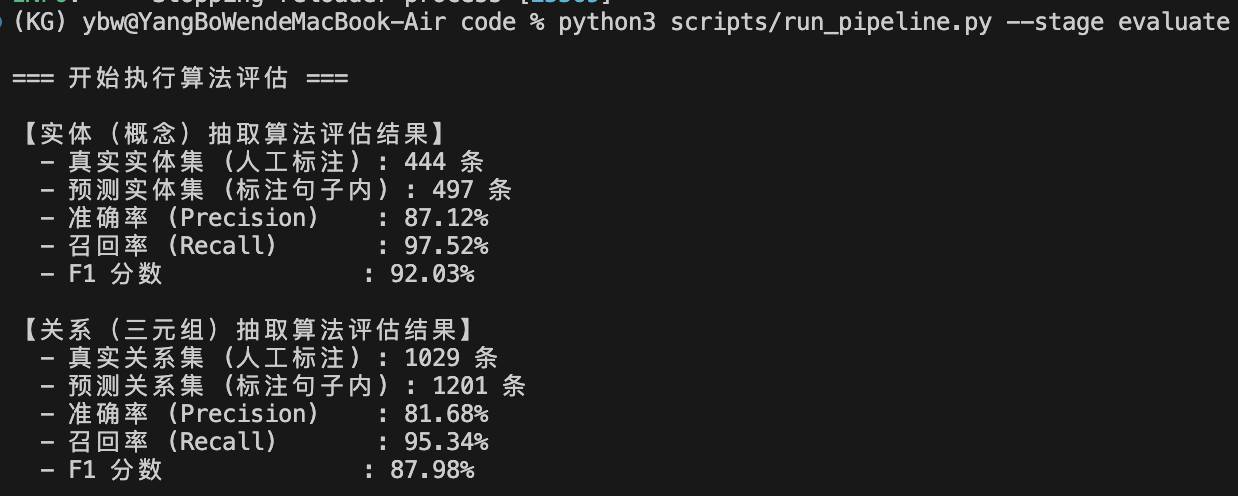
\includegraphics[width=0.82\textwidth]{figures/算法评估结果终端.png}
\caption{算法评估脚本终端运行输出结果}
\label{fig:terminal}
\end{figure}


从方法效果看，项目采用的混合方案在保持较高召回率的同时，通过术语清洗、实体二次过滤与关系多重约束提高了结果精度。说明“统计发现 + LLM 定稿 + 规则抽取”的路线在课程实验条件下具有较好的实用性和可解释性。

\subsection{算法评估结论}
综合两项任务的评估结果可以看出，实体抽取整体优于关系抽取。其主要表现为：实体抽取的 Precision、Recall 与 F1 均高于关系抽取，尤其是在 F1 指标上高出约 4 个百分点。造成这一差异的原因主要在于，实体抽取更多依赖术语词典、最长匹配和类型校验等相对稳定的规则，边界更明确、语义歧义相对较少；而关系抽取不仅依赖实体识别结果，还需要进一步判断两个实体之间是否真正存在稳定语义联系，因此更容易受到句式差异、触发词多义性和上下文复杂性的影响。

从系统定位看，这组实验结果说明本项目已经能够较稳定地支持变构飞行器领域知识的结构化组织任务。实体层面的高召回和高 F1 表明系统适合承担领域术语汇聚、概念归类和节点构建等基础工作；关系层面的较好表现则说明该系统已经具备构建初步语义连接网络的能力。虽然在复杂关系判定方面仍有进一步提升空间，但作为课程级领域知识组织原型，本系统已经能够较好地支撑知识图谱构建、可视化展示和后续扩展分析。

\subsection{误差来源与讨论}
从实体抽取结果看，召回率达到 97.52\%，说明术语词典与规则补充机制对领域概念具有较强覆盖能力，大部分人工标注实体能够被系统成功识别。Precision 为 87.12\%，略低于 Recall，说明当前词典匹配策略在保持高覆盖率的同时，也引入了少量假阳性实体。这类错误往往来自两个方面：一是部分通用术语在特定上下文中并非真正的领域实体，但仍被词典命中；二是个别短词项存在语义歧义，在句子中被错误识别为实体。

进一步分析可知，实体抽取误差与领域文献的表达复杂度密切相关。航空航天文献中存在大量带修饰语的复合术语、参数符号与自然语言混合表达、中文术语与英文缩写交替出现等现象，这些都容易造成实体边界不稳定。例如某些术语在一处以完整概念出现，而在另一处仅以简称出现，若别名映射覆盖不足，就可能产生重复识别或边界截断问题。此外，部分实体同时兼具概念属性和参数属性，其类型判断需要依赖上下文，而当前规则体系对这类细粒度歧义的区分能力仍有限。

从关系抽取结果看，Recall 达到 95.34\%，说明基于触发词的关系抽取机制能够较充分覆盖人工标注关系；但 Precision 为 81.68\%，低于实体抽取结果。这表明关系抽取比实体抽取更容易受到语义复杂性的影响。其主要原因在于：第一，同一句中两个实体虽然被触发词连接，但未必构成真正稳定的语义关系；第二，部分触发词如“基于”“采用”“影响”等在不同句式中语义范围较宽，容易引发过抽取；第三，当前方法主要面向句内显式关系，对隐式关系和复杂长距离关系的处理能力仍有限。

关系抽取的误差还反映出领域知识表达中“形式接近但语义不同”的典型问题。例如“某方法用于分析某参数变化”与“某参数影响某性能”在表层上都可能出现“用于”“影响”等触发词，但其真实语义角色并不相同。如果仅依赖浅层触发模式，很容易将方法关系、影响关系和适用关系相互混淆。此外，一些结构组成关系在句子中可能以列举方式出现，若缺少更强的依存约束或枚举边界识别，也可能将并列实体错误地连接为关系对。

从实验设计角度看，人工金标准本身也会对误差分析带来一定影响。目前标注集虽然已经能够反映系统总体效果，但在规模和覆盖面上仍有进一步扩展空间。尤其是在复杂长句、跨句承接、术语缩写和嵌套结构较多的样本上，如果标注数量进一步增加，将更有利于发现系统在边缘场景中的局限性。未来若能建立分层标注集，例如区分基础实体、复杂实体、显式关系和隐式关系，将有助于开展更细粒度的误差定位与模块优化。

总体而言，本项目在实体抽取和关系抽取两项任务上均取得了较好的实验结果，其中实体抽取 F1 达到 92.03\%，关系抽取 F1 达到 87.98\%，说明系统已经能够较稳定地支持变构飞行器领域知识图谱的构建任务。未来若进一步引入上下文建模、更细粒度的实体歧义消解策略以及轻量关系分类模型，预计仍有提升空间。


\newpage
\section{项目实践收获}
\subsection{项目实践收获}
通过本次课程大作业，我们系统体验了知识图谱从语料处理到应用展示的完整工程流程。相比只停留在单一算法实现，本项目让我们更加认识到知识图谱系统本质上是一项系统工程，具体收获如下：

\begin{itemize}[leftmargin=2em, itemsep=0.5ex]
    \item \textbf{数据治理层面：} 建立并强化了“数据治理先于知识建模”的工程意识。实践证明，PDF 文本抽取、乱码处理与标准化清洗才是决定后续抽取上限的基础。
    \item \textbf{知识建模层面：} 体会到领域本体设计是一个在“语义表达能力”与“工程可实现性”之间动态权衡的过程，训练了我们在复杂任务中进行抽象建模与粒度控制的能力。
    \item \textbf{团队协作层面：} 深入理解了工程任务中模块化拆分、接口对齐与并行开发的重要性，双人协作模式有效提高了联调效率与问题定位速度。
    \item \textbf{系统实现层面：} 分层流水线的设计显著提升了系统的可维护性与可复现性，使我们学会了如何构建符合真实项目思路的可迭代工程架构。
    \item \textbf{实验评估层面：} 认识到从“做出系统”走向“证明有效”的重要性。只有通过构建金标准并进行定量分析，才能真正明确一个图谱系统的性能边界。
\end{itemize}

\subsection{项目特色与创新点}
本项目的特色与创新主要体现在以下几个方面：
\begin{enumerate}[leftmargin=2.2em,label=\arabic*.]
    \item \textbf{完整的工程闭环。} 项目并非只关注某一个局部算法，而是实现了从文献获取、文本预处理、术语抽取、实体关系抽取、图谱构建、多格式导出到前端可视化和算法评估的完整闭环。这种从“数据—算法—系统—实验”全链条展开的组织方式，使项目更接近实际工程原型，而不是停留在单点功能演示层面。
    \item \textbf{较强的规范性。} 项目采用模块化目录结构和标准化中间文件格式，统一使用 \texttt{jsonl}、\texttt{csv}、\texttt{json} 和 \texttt{ttl} 等格式保存中间结果与最终结果。同时引入人工金标准、Precision、Recall 和 F1 等标准评价方式，对知识抽取效果进行量化分析，从而保证整个系统具备较好的可复现性与可解释性。
    \item \textbf{“全自动发现 + 人工介入优化”双模混合知识构建方法。} 本项目提出并实现了这一双轨式知识构建方案。一方面，系统支持基于统计特征（TF-IDF/PMI）与 LLM 语义精筛的全自动知识发现流水线，能够快速处理海量无标注文献；另一方面，系统能够无缝检测并融合人工构建的实体词典与金标准三元组，并利用人工标注集对自动模型进行动态评估与针对性优化。这种方案既保留了大规模抽取的高召回率，又通过人工金标准的引入确保了核心知识的高度精准，充分体现了“机器发现、人工辅助、指标驱动”的现代知识图谱构建思想。
    \item \textbf{面向中文 PDF 的容错处理流程。} 针对中文学术 PDF 常见的乱码、文本层异常和扫描页问题，项目设计了“文本层抽取—细粒度回退—OCR 兜底”的多级容错处理流程；针对关系抽取易产生伪三元组的问题，引入触发词位置、实体黑名单、距离阈值和类型约束四重过滤机制。这些设计直接面向真实文档噪声和抽取误差来源，具有较强工程针对性。
    \item \textbf{轻量化可视化展示方案。} 项目构建了基于 FastAPI 与 ECharts 的轻量化知识图谱可视化系统，无需依赖复杂图数据库即可完成图谱展示、搜索、筛选和详情查看。该实现方式显著降低了部署与演示门槛。
\end{enumerate}
综合来看，本项目的特色与创新并不体现在某一个单独模型上，而体现在面对真实领域文献时所形成的一套完整、规范、可展示、可扩展的知识图谱原型方案。

\subsection{项目不足与改进方向}
尽管本项目已经完成了较完整的知识图谱原型系统，但从更高标准的研究和工程应用要求来看，仍然存在若干不足。首先，在实体识别方面，当前方法仍以词典匹配和规则补充为主，对新术语自动发现能力有限。当文献中出现未被术语表覆盖的新概念、缩写变体或上下文依赖较强的表达时，系统可能出现漏识别或类型判断不稳定的问题。尤其对于嵌套实体、长复合术语和带参数修饰的短语，现有方法仍有进一步优化空间。

其次，在关系抽取方面，虽然系统已经引入了大语言模型辅助处理复杂长难句中的隐式关联，但在极端长文本跨段落的推理上仍有局限。变构飞行器领域文献中经常出现跨段落嵌套、长篇并列列举和分散于不同章节的多实体逻辑共现。目前的并发批处理策略容易产生上下文截断，导致超出单次批处理窗口的因果逻辑链条断裂。因此，未来应考虑引入 RAG（检索增强生成）技术、图神经网络推理算法或更长上下文窗口的专用模型，以实现跨篇章级别的深度关系发现。

在系统应用层面，目前前端已具备基本的图谱展示、搜索和筛选能力，但尚未进一步扩展到路径分析、语义问答、关系推荐和知识演化分析等更高层次功能。若后续将图谱与图数据库、问答系统或推理模块结合，系统可从“展示型原型”逐步演进为“分析型工具”。此外，当前图谱更新流程仍以离线批处理为主，若未来加入增量更新机制与版本管理能力，将更有利于长期维护和持续扩充。

综合来看，本项目的后续改进方向可以概括为两个层面：一是增强抽取层的上下文理解能力，提高对复杂实体和复杂关系的处理效果；二是拓展应用层的交互分析与智能服务能力，使知识图谱从课程级展示系统逐步走向更具实用价值的领域知识服务平台。

\subsection{小组成员分工明细}
本项目由两人小组共同完成，双方在算法设计、系统开发与报告撰写上紧密配合，工作量均等。具体分工明细如表~\ref{tab:division} 所示。

\begin{table}[H]
\centering
\caption{小组成员分工明细}
\label{tab:division}
\renewcommand{\arraystretch}{1.3}
\resizebox{\textwidth}{!}{%
\begin{tabular}{>{\centering\arraybackslash}p{2.5cm}>{\centering\arraybackslash}p{3cm}>{\raggedright\arraybackslash}p{8cm}>{\centering\arraybackslash}p{2cm}}
\toprule
姓名 & 学号 & 负责核心工作内容 & 贡献比例 \\
\midrule
杨博文 & 3023244317 & $\bullet$ 需求分析与技术方案设计 \newline $\bullet$ 领域文献收集与文本清洗 \newline $\bullet$ 术语提取（统计特征 + LLM 精筛） \newline $\bullet$ 实体关系抽取规则设计 \newline $\bullet$ 人工金标准构建与效果评估 \newline $\bullet$ 技术报告联合撰写与修订 & 50\% \\
\midrule
于露雪 & 3023244303 & $\bullet$ 系统架构设计与工程部署 \newline $\bullet$ PDF 文本提取与容错模块 \newline $\bullet$ 大模型并行抽取与词典增量逻辑 \newline $\bullet$ FastAPI 后端开发与图谱多格式导出 \newline $\bullet$ ECharts 前端交互系统开发 \newline $\bullet$ 技术报告主笔与排版 & 50\% \\
\bottomrule
\end{tabular}%
}
\end{table}

\subsection{总结}
本文围绕“变构飞行器领域知识图谱构建与可视化系统设计与实现”这一题目，完成了领域数据整理、文本预处理、术语构建、实体关系抽取、图谱导出、可视化展示和评估分析等关键任务。整体上，本项目已经实现了一个具有较好完整性、规范性和一定创新性的课程原型系统。


\newpage
\section{致谢}
值此课程大作业顺利结项与本技术报告完稿之际，我们谨向在项目推进与系统研发过程中给予支持和帮助的各位师长致以诚挚的谢意。

首先，特别感谢饶老师在本学期课程中的悉心授课。饶老师在课堂上对知识图谱核心理论的深入剖析与对前沿技术的生动讲解，为我们完成本次大作业打下了坚实的理论基础。正是由于老师严谨求实的治学态度与专业的学术引领，才使得我们能够理清知识发现、本体建模与关系抽取的本质，并最终顺利将课本知识转化为实际的工程原型系统。

其次，衷心感谢本课程的各位助教在日常答疑、作业批改以及实验环境配置等环节所付出的辛勤劳动。助教团队的耐心解答与技术支持，为我们跨越工程实现初期的技术壁垒提供了极大帮助，有力保障了本项目的顺利推进。

最后，感谢学校及学院开设本门课程，为我们搭建了从基础理论迈向工程实践的广阔平台。本次大作业不仅深化了我们对知识获取、本体建模及图谱可视化等核心技术的理解，更全面锤炼了我们在复杂系统开发、问题边界探索以及规范化学术表达等方面的综合科研能力。

受限于现有学术水平与开发时间，本系统及报告中不可避免地存在亟待完善之处。我们将以此次项目为契机，在未来的学习与科研道路上秉持严谨求真的精神，继续探索、砥砺前行。


\end{document}
